\documentclass[fontsize=11pt]{../common/thesis}

\usepackage[T1]{fontenc}
% \usepackage[sfdefault]{roboto}
\usepackage{libertine}
\usepackage[libertine,cmintegrals,cmbraces,vvarbb]{newtxmath}
\usepackage{wrapfig}
\usepackage{../common/adpwrapfig}

% PDF and title properties.
\SgSetTitle{On Efficient Training \& Inference of Neural Differential Equations}
\SgSetTitleSplitOne{On Efficient Training \& Inference of Neural Differential}
\SgSetTitleSplitTwo{Equations}
\SgSetAuthor{Avik Pal}
\SgSetYear{2022}
\SgSetDegree{Master of Science}
\SgSetDepartment{Department of Electrical Engineering and Computer Science}
\SgSetUniversity{Massachusetts Institute of Technology, Cambridge, Massachusetts}
\SgSetCompletionDate{May 19, 2023}
\SgSetLab{CSAIL}
\SgSetAddrLineOne{32-G785, Julia Lab, Stata Center}
\SgSetAddrLineTwo{Cambridge, MA, 02139}
\SgSetBriefProblemStatement{}
\SgSetAdvisor{Alan Edelman}
\SgSetAdvisorRole{Professor}
\SgSetAdvisorDept{Department of Mathematics}

% Remove Chapter Numbering
\renewcommand\thesection{\arabic{section}}

\usepackage{pifont}% http://ctan.org/pkg/pifont
\usepackage{xcolor}%
\usepackage{mathtools}%
\usepackage{subcaption}
\usepackage{caption}
\usepackage{adjustbox}
\usepackage{arydshln}
\usepackage{tabularx}
\usepackage{makecell}
\usepackage{lipsum}
\usepackage{algorithm}
\usepackage{algpseudocode}
\usepackage{minted}
\usepackage{textgreek}

% \mathtoolsset{showonlyrefs=true} % show only crossref-ed equation numbers

% Markers
\newcommand{\cmark}{\ding{51}}%
\newcommand{\xmark}{\ding{55}}%
\newcommand{\crossmark}{{\color{red} \xmark}}%
\newcommand{\tickmark}{{\color{green} \cmark}}%

% Citations
\newcommand{\tocite}{{\color{blue} \textbf{[citation needed]}}}
\newcommand{\tocitex}[1]{{\color{blue} \textbf{[citation needed: #1]}}}

% Todonotes alternatives
\newcommand{\todo}[1]{{\color{orange} (\textbf{todo}) #1}}
\newcommand{\note}[1]{{\color{purple} (\textbf{note}) #1}}
\newcommand{\avik}[1]{{\color{red} (avikpal@) #1}}
\newcommand{\cred}[1]{{\color{red}#1}}

\newcommand{\stcopy}{{\color{green} Done (Copy)}}
\newcommand{\stwip}{{\color{orange} WIP}}
\newcommand{\sttodo}{{\color{red} Todo}}
\newcommand{\stdone}{{\color{green} Done}}
\newcommand{\stblock}{{\color{red} Blocking}}
\newcommand{\stnblock}{{\color{purple} Non Blocking}}

% Reporting results
\newcommand{\sdval}[2]{$#1 \pm #2$}
\newcommand{\sdvalb}[2]{$\mathbf{#1 \pm #2}$}

% Horizontal Phantom Shortcut
\newcommand{\hp}[1]{\hphantom{#1}}

% ax - bx
\newcommand{\timeschange}[2]{$\mathit{#1\times - #2\times}$}

% Differential Equations
\newcommand{\atol}{\texttt{atol}}
\newcommand{\rtol}{\texttt{rtol}}
\newcommand{\eest}{\texttt{E}_{\texttt{Est}}}
\newcommand{\sest}{\texttt{S}_{\texttt{Est}}}
\newcommand{\treg}{\texttt{t}_{\texttt{reg}}}
\newcommand{\dt}{\mathrm{d}t}

% Math Helpers
\newcommand{\func}[2]{#1\left(#2\right)}
\newcommand{\funct}[2]{\texttt{#1}\left(#2\right)}
\newcommand{\cprob}[3]{\func{#1}{#2~\mid~#3}}
\newcommand{\prob}[2]{\func{#1}{#2}}
\newcommand{\Exp}[2]{\mathbb{E}_{#1}\left[{#2}\right]}

% Complexity Notations
\newcommand{\bigO}[1]{\func{\mathcal{O}}{#1}}

% Copied from a paper
\newcommand{\cpaper}{~$^\text{\textparagraph}$}

% Footnote without marker
\newcommand\blfootnote[1]{%
  \begingroup
  \renewcommand\thefootnote{}\footnote{#1}%
  \addtocounter{footnote}{-1}%
  \endgroup
}

% Colored lipsum
\newcommand{\clipsum}[1]{{\color{purple} \lipsum[#1]}}

% DEQs
\newcommand{\zstar}{z^*}

% Change Numbering
\renewcommand\thesection{\thechapter.\arabic{section}}
\renewcommand\thesubsection{\thesection.\arabic{subsection}}
\renewcommand\thesubsubsection{\thesubsection.\arabic{subsubsection}}
\renewcommand\thealgorithm{\thechapter.\arabic{algorithm}}

\renewcommand\thesubfigure{\thefigure.\arabic{subfigure}}

% Unicode Character
\DeclareUnicodeCharacter{2202}{\ensuremath{\partial}}

% Minted
\usemintedstyle{xcode}

% The document.
\begin{document}

\begin{frontmatter}
  \SgAddTitle%
  \begin{abstract}
  
\end{abstract}%
  \chapter*{Originality}

The writing of this thesis is my original work. The material in this thesis is either my original work with or without collaborators, or is based on the work of others duly cited.

\section*{Publications}

This thesis contains materials from the following publications/pre-prints listed in chronological order:

\textbf{Opening the Blackbox: Accelerating Neural Differential Equations by Regularizing Internal Solver Heuristics}\\
Avik Pal, Yingbo Ma, Viral Shah, Chris Rackauckas\\
\textit{International Conference on Machine Learning (ICML)}, 2021.

\textbf{Continuous Deep Equilibrium Models: Training Neural ODEs Faster by Integrating Them to Infinity}\\
Avik Pal, Alan Edelman, Chris Rackauckas\\
\textit{arXiv preprint arXiv:2201.12240}, 2022.

\textbf{Locally Regularized Neural Differential Equations: Some Black Boxes Were Meant to Remain Closed!}\\
Avik Pal, Alan Edelman, Chris Rackauckas\\
\textit{International Conference on Machine Learning (ICML)}, 2023.

\section*{Open Source Software}

A substantial part of my Masters was dedicated to writing and contributing open source software. I believe these software have enabled other researchers and practitioners to build upon my work and help accelerate the pace of research in the field of scientific machine learning. The following are the open source software that I have written:

\textbf{Lux.jl}: Explicitly Parameterized Neural Networks in Julia\\
{\small \url{https://github.com/LuxDL/Lux.jl}}

\textbf{DeepEquilibriumNetworks.jl}: Fast Discrete and Continuous Deep Equilibrium Networks\\
{\small \url{https://github.com/SciML/DeepEquilibriumNetworks.jl}}

\section*{Breakdown of Contributions}

\citet{pal2022mixing} and \citet{pal2023locally} were written and published during my Masters at MIT. \citet{pal2021opening} was published prior to me joining MIT and it has been included in my thesis to provide a coherent story about acceleration of Neural Differential Equations, since a detailed discussion on \citet{pal2023locally} is not possible without the preceding version of the paper~\citep{pal2021opening}.

All the software mentioned above were written during my Masters at MIT. \textit{Lux.jl} development was heavily inspired by my prior experience in developing \textit{Flux.jl}~\citep{innes:2018, innes2018fashionable}. \textit{DeepEquilibriumNetworks.jl} was written as a part of my research on \citet{pal2022mixing}. 
%  % Can also move to introduction
  \chapter*{Acknowledgement}

I would like to express my sincere gratitude and appreciation to all those who have supported and contributed to the completion of my master's thesis. Without their invaluable assistance, encouragement, and guidance, this research would not have been possible.

First and foremost, I am deeply indebted to my thesis advisors, Dr. Alan Edelman and Dr. Chris Rackauckas, for their unwavering support, patience, and expertise throughout this journey. Their insightful feedback, constructive criticism, and constant encouragement played a pivotal role in shaping the direction and quality of this thesis. I am truly grateful for their mentorship and the invaluable lessons I have learned under their guidance.

I am also thankful to my peers at the Julia Lab CSAIL and the broader EECS MIT community, who provided a nurturing academic environment that facilitated my research endeavors. Their commitment to excellence and dedication to fostering intellectual growth have been instrumental in shaping my academic development. I extend my heartfelt appreciation to all my professors, colleagues, and peers who engaged in thought-provoking discussions, provided valuable feedback, and offered their support.

My gratitude extends to my parents, Abhijit Pal and Rupa Pal, for their unwavering love, belief in my abilities, and constant encouragement. They have been my pillars of strength throughout this journey. I am especially thankful to my brother, Dr. Aritra Pal, whose motivation to pursue a Ph.D. program paved the way for my academic journey. Without their constant support, understanding, and encouragement, this work would not have been possible.

Completing this master's thesis has been a challenging yet rewarding journey, and I feel truly honored to have had the opportunity to undertake this research. The support and contributions of everyone mentioned above have been pivotal in making this thesis a reality. I express my deepest gratitude to all for their unwavering support, belief in my abilities, and for being an integral part of this significant milestone in my academic and personal life.%
  \SgAddToc%  Table of contents.
  \SgAddLof%  List of figures.
  \SgAddLot%  List of tables.
  \SgAddLoa%  List of algorithms.
\end{frontmatter}

% Introduction
\chapter{Introduction}
\label{chapter:introduction}

The combination of numerical methods and scientific computing with machine learning holds immense potential for democratizing the field. Developing neural network architectures that automatically adapt to new problems is crucial in advancing machine learning algorithms. How many hidden layers should you choose in your recurrent neural network? \citet{chen2018neural} showed that the answer could be found automatically by using a continuous reformulation, the neural ordinary differential equation, and allowing an adaptive ODE solver to effectively choose the number of steps to take. Explicit models maximize performance on a dataset by being tuned to the ``hardest'' training sample, which hurts the inference timings for ``easier'' -- more abundant -- samples. Using adaptive differential equation solvers allows these implicit models to choose the number of steps they need effectively. Additionally, these models have constant memory overhead for training, i.e., irrespective of the number of steps of the solver, backpropagation takes constant memory.

Implicit Machine Learning has emerged as a popular modeling framework, enabling ML practitioners to design neural networks that can adaptively modify their depth based on the input problem. The ``depth'' of these models is typically a function of the number of internal explicit neural network evaluations. In this thesis, we will focus on two main types of implicit models -- Deep Equilibrium Models (DEQs)~\citep{bai_deep_2019} drive a discrete dynamical system parameterized by a neural network to steady state, and Neural Ordinary Differential Equations (Neural ODEs)~\citep{chen2018neural} solve an ODE parameterized by a neural network over a fixed time-span. There are several extensions/generalizations to these frameworks -- like Multiscale DEQs~\citep{bai_multiscale_2020}, Neural Stochastic Differential Equations~\citep{liu2019neural}, Universal Differential Equations~\citep{rackauckas2020universal}, etc. -- and we will show that our proposed methods naturally extend to these setups.

However, there is no free lunch. Despite much research in this domain, one fact remained: \textit{solving a neural differential equation is expensive, and training a neural differential equation is even more so}. \citet{grathwohl2018ffjord, dupont2019augmented, kelly2020learning, finlay2020train} have identified several problems with training implicit networks. Implicit Models come with extremely high training and inference costs making them not as scalable as explicit models like transformers~\citep{chen2016attention, vaswani2017attention}, recurrent neural networks~\citep{elman1990finding, hochreiter1997long}, etc. Accelerating forward pass is as simple as demanding the solver to ``take fewer steps.'' But this ``simple objective'' is non-differentiable. Several solutions have been proposed using proxy losses for this objective -- \citet{kelly2020learning, finlay2020train} use higher order derivatives for regularization of Neural Differential Equations, \citet{pal2021opening} proposed a ``zero-cost'' global regularization scheme for problems using adaptive differential equation solvers, and \citet{bai2021stabilizing} use jacobian regularization for Deep Equilibrium Models. Other alternate strategies have been learning new solvers~\citep{poli2020hypersolvers}, randomizing the timespan for integration to smoothen the learned dynamics~\citep{ghosh2020steer}. We build upon prior works to  propose a generally applicable Neural ODE regularization scheme and a infinite time Neural ODE which provide faster training and inference compared to existing methods.

\section{Outline of the Thesis}

In \Cref{part:foundations}, we describe the background needed to understand the novel methods proposed in this thesis. \Cref{chapter:neural_ode} describe the background on Ordinary Differential Equations and Neural Ordinary Differential Equations. \Cref{chapter:deep_equilibrium_models} describes the background on Deep Equilibrium Models or Infinite Depth Neural Networks. We describe our methods in \Cref{part:accelerating_nde}. \Cref{chapter:infinite_time_neural_odes} introduces Infinite-Time Neural ODEs which accelerate the training of Neural ODEs by integrating them to infinity. In \Cref{chapter:internal_solver_heuristics_regularized_neural_des} we open black box differential equation solvers and use internal solver heuristics and discrete sensitivity analysis to accelerate the training and inference of Neural Differential Equations. In \Cref{chapter:local_regularization_neural_odes} we observe the shortcomings of former global regularization schemes and propose a local regularization scheme for Neural ODEs. In \Cref{part:open_source_software}, we describe the open-source softwares developed as a part of this thesis work. Finally we conclude the thesis with open future research directions in \Cref{part:conclusion_and_future_work}.

\section{Main Contributions}

The main contributions of this thesis are as follows:
%
\begin{enumerate}
  \item In \Cref{chapter:infinite_time_neural_odes}, we will design a \textit{continuous variant of Deep Equilibrium Networks} that is equivalent to integrating a Neural ODE to \textit{infinite}.
  \item In \Cref{chapter:infinite_time_neural_odes}, we will demonstrate empirically and mathematically that \textit{integrating a Neural ODE to infinity} accelerates the backwards pass.
  \item In \Cref{chapter:internal_solver_heuristics_regularized_neural_des}, we will build upon the internals of differential equation solvers and open the solver black-box to \textit{accelerate training and inference of Neural Differential Equations}.
  \item In \Cref{chapter:local_regularization_neural_odes}, we will further show that trading off slight performance allows us to develop a \textit{highly-composable stochastic local regularization scheme} for Neural Differential Equations.
  \item In \Cref{chapter:lux_bridging_scientific_computing_and_deep_learning}, we introduce a new Julia deep learning library, \textit{Lux}, that bridges the gap between scientific computing and deep learning.
\end{enumerate}


% Background
\part{FOUNDATIONS}
\label{part:foundations}

\chapter{Neural Ordinary Differential Equations}
\label{chapter:neural_ode}

\section{Ordinary Differential Equations}
\label{sec:ordinary_differential_equations}

Ordinary Differential Equations (ODEs) are equations defined by a relationship to its derivative. We can generally write an ODE as:
%
\begin{equation}
  \frac{\partial z}{\partial t} = \func{f}{z, p, t}
\end{equation}
%
This effectively describes the evolution of a state $\func{z}{t}$. To compute $\func{z}{t}$, we could solve the following integral equation:
%
\begin{equation}
  \func{z}{t} = \int_{t_0}^{t} \func{f}{z, p, t} \, \dt
\end{equation}
%
where $t_0$ is the initial time. However, computing these solutions analytically is almost impossible and hence we need to rely on numerical solvers. For this thesis, we will focus exclusively on Initial Value Problems (IVP) which specify the differential equations along with an initial condition, i.e., value of the state at $t_0$: $z(t_0)$. There are other kinds of ODE Problems like Boundary Value Problems (BVP) which specify additional conditions at the end of the interval, i.e., $z(t_1)$.

Numerical Solvers for ODEs can be broadly categorized into Implicit Methods and Explicit Methods. Explicit Methods compute the state of the dynamical system at a future time-point given the current state. Implicit Methods solve for the the state of the dynamical system at a future time-point given the current state \textit{and the later one}. For example, consider two extremely simple numerical solvers for an ODE:
%
\begin{itemize}
  \item Euler Method (Explicit Method)~\citep{euler1824institutionum}:
        %
        \begin{equation}
          z_{n + 1} = z_n + \dt \cdot \func{f}{z_n, p, t_n}
        \end{equation}
        %
  \item Backward Euler Method (Implicit Method)~\citep{euler1824institutionum}:
        %
        \begin{equation}
          z_{n + 1} = z_n + \dt \cdot \func{f}{z_{n + 1}, p, t_{n + 1}}
        \end{equation}
        %
\end{itemize}
%
Explicit methods tend to be faster than implicit methods but are not effective for solving stiff equations~\citep{wanner1996solving,kim2021stiff}. In this thesis, we will exclusively use explicit methods. A detailed discussion on implicit and explicit methods is beyond the scope of this thesis and we refer the readers to \citet{rackauckas2019scimlbook}.

\section{Explicit ODE Solvers}
\label{subsec:explicit_ode_solvers}

In this section, we will briefly discuss ODE solvers that are relevant in the context of Neural ODEs. We start with Euler Method~(\Cref{subsec:euler_method}) to give a simple introduction to numerical solvers. Then we build upon that to describe the Tsitouras $\mathbf{5 (4)}$ Runge-Kutta Method~(\Cref{subsec:tsit5_method}) that servers as an excellent default for most ODEs at lower tolerances. Finally we describe $\mathbf{3^{rd}}$ order Adams-Bashforth Method~(\Cref{subsec:vcab3_method}), a multi-step method that we find to be particularly useful for Neural ODEs.

\subsection{Euler Method}
\label{subsec:euler_method}

The forward Euler method is one of the simplest methods to numerically solve an IVP. Consider the Taylor series expansion of the function $\func{z}{t}$ around $t_n$:
%
\begin{equation}
  \func{z}{t + \dt} = \func{z}{t} + \dt \cdot \left. \frac{\partial z}{\partial t} \right|_{t} + \frac{1}{2} \dt^2 \cdot \left. \frac{\partial^2 z}{\partial t^2} \right|_{t} + \bigO{\dt^3}
\end{equation}
%
If we ignore the quadratic and higher order terms, we get the forward Euler method~\citep{euler1824institutionum}:
%
\begin{align}
  & \func{z}{t + \dt} = \func{z}{t} + \dt \cdot \left. \frac{\partial z}{\partial t} \right|_{t}\\
  \implies & z_{n + 1} = z_n + \dt \cdot \func{f}{z_n, p, t_n}
\end{align}
%
This method is extremely simple however, has an extremely high local truncation error of $\bigO{\dt^2}$. Hence, this method is rarely used in the context of most IVPs and especially not for Neural ODEs.

\subsection{Tsitouras $\mathbf{5 (4)}$ Runge-Kutta (Tsit5) Method}
\label{subsec:tsit5_method}

Runge-Kutta (RK) Methods~\citep{runge1895numerische, kutta1901beitrag} are widely used to approximate the solutions of ODEs numerically. Given a tableau of coefficients $\left\{A, c, b\right\}$, these methods combine $s$ stages to obtain the estimate at $t + \dt$.
%
\begin{align}
    & k_s = \func{f}{t + c_s \cdot \dt, z(t) + \sum_{i = 1}^{s - 1} a_{si} \cdot k_i}\\
    & z(t + dt) = z(t) + \dt \cdot \left( \sum_{i = 1}^s b_i \cdot k_i \right)
\end{align}
%
\citet{tsitouras2011runge} presented a tableau of coefficients for a 6-stage RK method of order $5 (4)$. We have found Tsit5 to be an excellent default for most ODEs (including Neural ODEs) at lower tolerances. \todo{pull up some results from SciMLBenchmarks}

\subsection{$\mathbf{3^{rd}}$ order Adams-Bashforth (VCAB3) Method}
\label{subsec:vcab3_method}

Contrary to RK Methods, Multi-step methods compute $\func{z}{t}$ by efficiently using the information from previous time-steps. A linear multi-step method uses a linear interpolation to compute $z_{n + 1}$:
%
\begin{equation}
  z_{n + 1} = z_n + \dt \cdot \sum_{i = 0}^{s} \beta_i \cdot \func{f}{z_{n + 1 - i}, p, t_{n + 1 - i}} \qquad \texttt{given } \sum_{i = 0}^s \beta_i = 1
\end{equation}
%
where $s$ is the number of steps. If $\beta_0 = 0$, then we have an explicit method. In this thesis, we will focus on Adams methods which involve solving:
%
\begin{equation}
  z_{n + 1} = z_n + \int_{t_n}^{t_{n + 1}} \func{f}{z(\tau), p, \tau} \cdot \mathrm{d}\tau
\end{equation}
%
Adams methods approximate the integral using polynomial interpolation of the function $f$ using evaluations at points $\left\{ t_{n + 1 - s}, t_{n + 2 - s}, \dots, t_{n} \right\}$. Adams-Bashforth Method approximates the function using Lagrange Interpolation:
%
\begin{equation}
  \func{f}{z(\tau), p, \tau} \approx \sum_{i = 0}^{s} \mathcal{L}_{n + 1 - i} \cdot \func{f}{z_{n + 1 - i}, p, t_{n + 1 - i}}
\end{equation}
%
where $\mathcal{L}_{n + 1 - i}$'s are the Lagrange polynomials. For $s = 3$, we get the $\mathbf{3^{rd}}$ order Adams-Bashforth (VCAB3) Method~\citep{durran1991third}:
%
\begin{equation}
  z_{n + 1} = z_n + \frac{\dt}{12} \cdot \left( 23 \func{f}{z_n, p, t_n} - 16 \func{f}{z_{n - 1}, p, t_{n - 1}} + 5 \func{f}{z_{n - 2}, p, t_{n - 2}} \right)
\end{equation}
%
This method has a local truncation error of $\bigO{\dt^3}$. Additionally, since this method evaluates $f$ very infrequently (by reusing the evaluations of $f$ from previous time-steps), it is efficient for ODEs with expensive evaluations of $f$ like a Neural ODE.

\section{Adaptive Time-Stepping in Numerical ODE Solvers}
\label{sec:adaptive_time_stepping}

\todo{might need rewording}

\todo{quite specific to RK methods. add comments for multistep methods}

Adaptive solvers need to maximize the step size ($\dt$) while keeping the error estimate below the user-specified tolerances, i.e., they need to satisfy:
%
\begin{equation}
    \eest \leq \atol + \texttt{max}\left( |z(t)|, |z(t + \dt)|\right) \cdot \rtol
\end{equation}
%
where $\eest$ is the local error estimate. Adaptive solvers utilize an additional linear combiner $\Tilde{b}_i$ to get an alternate solution, typically with one order less convergence~\citep{wanner1996solving, fehlberg1968classical, dormand1980family,tsitouras2011runge}.
%
\begin{equation}
  \Tilde{z}(t + dt) = z(t) + \dt \cdot \left( \sum_{i = 1}^s \Tilde{b}_i \cdot k_i \right)
\end{equation}
%
A classic result from Richardson extrapolation shows that $\eest = \| \Tilde{z}(t + \dt) - z(t + \dt) \|$ is an estimate of the local truncation error~\citep{hairer1, ascher1998computer}. The new step size is determined using the following:
%
\begin{equation}
    q = \left\| \frac{\eest}{\atol + \texttt{max}\left( |z(t)|, |z(t + \dt)|\right) \cdot \rtol} \right\|
\end{equation}
%
\begin{itemize}
    \item If $q < 1$, $\dt$ is accepted.
    \item Otherwise, it is rejected and reduced. A standard PI controller proposes the new step size to be:
    %
    \begin{equation}
        dt_{new} = \eta \cdot q_{n - 1}^\alpha \cdot q_{n}^\beta \cdot dt
    \end{equation}
    %
    where $\eta$ is the safety factor, $q_{n - 1}$ is the error proportion of the previous step, and $(\alpha, \beta)$ are tunable PI-gain hyperparameters~\cite{wanner1996solving}. 
\end{itemize}

We defer the discussion of error estimation schemes for stochastic RK integrators to  \citet{rackauckas2017adaptive, rackauckas2020sosri}.

\todo{do a section on error estimation for stochastic RK integrators in Neural SDEs chapter}


\section{Sensitivity Analysis of ODEs}
\label{sec:sensitivity_analysis_odes}

\subsection{Continuous Sensitivity Analysis}
\label{subsec:continuous_sensitivity_analysis_odes}

\subsection{Discrete Sensitivity Analysis}
\label{subsec:discrete_sensitivity_analysis_odes}


\section{Neural Ordinary Differential Equations}
\label{sec:neural_odes}

% \section{Not All ODE Solvers are Created Equal}
% \label{sec:not_all_solvers_are_created_equal}

% \todo{Show a plot from SciMLBenchmarks.jl to emphasize why we need multiple kinds of solvers even for Neural ODEs.}

\section{Common Applications of Neural ODEs}
\label{sec:neural_odes_applications}

\subsection{Continuous Alternative to Residual Networks}
\label{subsec:continuous_alternative_to_residual_networks}

\subsection{Density Estimation: Continuous Normalizing Flows and FFJORD}
\label{subsec:density_estimation_neural_odes}

\subsection{Time Series Predictions}
\label{subsec:time_series_predictions}

\section{Accelerating Neural ODEs}
\label{sec:accelerating_neural_odes_prior_works}

\subsection{Jacobian Regularization FFJORD}

\subsection{Taylor Neural ODE}

\subsection{STEER}

\subsection{Hypersolvers for Neural ODEs}

\subsection{Opening the Blackbox: Global Regularization Schemes}

% \chapter{Neural Stochastic Differential Equations}
\label{chapter:neural_stochastic_differential_equations}
\chapter{Deep Equilibrium Models}
\label{chapter:deep_equilibrium_models}

\section{Steady State Problems}
\label{sec:steady_state_problems}

Steady State Problems involve determining the equilibrium state of a system, i.e., the state of the system where the rate of change of the system is zero. Let, our steady state problem be defined as follows:
%
\begin{equation}
  \frac{dz}{dt} = \func{f_\theta}{z, t} - z \label{eq:steady_state_problem}
\end{equation}
%
In the case of continuous dynamical systems, the steady state would be determined by the partial derivative w.r.t. time being zero:
%
\begin{equation}
  \frac{dz}{dt} = 0 \label{eq:steady_state_continuous}
\end{equation}
%
In case of discrete dynamical systems, the steady state would be defined by states remaining constant over time:
%
\begin{equation}
  z_{n + 1} = z_n \implies \zstar = \func{f_\theta}{\zstar, \infty} \label{eq:steady_state_discrete}
\end{equation}
%
There are two ways to solve steady-state problems:
%
\begin{enumerate}
  \item \textbf{Treating it as a Nonlinear Problem}: Steady State Problems can be efficiently solved by Nonlinear Solvers by removing the temporal dependence of the function $f_\theta$ with $\infty$. This is typically the most efficient way to solve steady state problems, however, it might give the non-preferred root. Solving this is equivalent to solving \Cref{eq:steady_state_discrete}.

  \item \textbf{Treating it as an ODE}: Another approach to solve steady state problems is to use the ODE form in \Cref{eq:steady_state_problem} with a time span of $(0, \infty)$ with a termination condition when \Cref{eq:steady_state_continuous} is satisfied. This approach is typically slower than the first approach, however, it respects the temporal dependence of the function $f_\theta$.
\end{enumerate}
%

% \todo{\url{https://docs.sciml.ai/NonlinearSolve/stable/solvers/SteadyStateSolvers/}}

\section{Sensitivity Analysis of Steady State Problems}
\label{sec:sensitivity_analysis_ssproblems}

Let, $\zstar$ be the steady state solution of the system, i.e., $\zstar = \func{f_\theta}{\zstar, \infty}$. For the sake of brevity, let us drop the $t = \infty$ term, i.e., $\zstar = \func{f_\theta}{\zstar}$. Differentiating w.r.t. $\theta$ we get:
%
\begin{align}
           & \frac{\partial \zstar}{\partial \theta} = \frac{\partial \func{f_\theta}{\zstar}}{\partial \zstar} \times \frac{\partial \zstar}{\partial \theta} + \frac{\partial \func{f_\theta}{\zstar}}{\partial \theta} \\
  \implies & \left( I - \frac{\partial \func{f_\theta}{\zstar}}{\partial \zstar} \right) \times \frac{\partial \zstar}{\partial \theta} = \frac{\partial \func{f_\theta}{\zstar}}{\partial \theta}
\end{align}
%
Let, the cost function we are optimizing be $\func{g}{\zstar, \theta}$. Taking the total derivative of $\func{g}{\zstar, \theta}$ w.r.t. the parameters $\theta$ we get:
%
\begin{align}
  \frac{d \func{g}{\zstar, \theta}}{d \theta} & = \frac{\partial \func{g}{\zstar, \theta}}{\partial \zstar} \times \frac{\partial \zstar}{\partial \theta} + \frac{\partial \func{g}{\zstar, \theta}}{\partial \theta}                                                                                                                                 \\
                                              & = \frac{\partial \func{g}{\zstar, \theta}}{\partial \zstar} \times \left( I - \frac{\partial \func{f_\theta}{\zstar}}{\partial \zstar} \right)^{-1} \times \frac{\partial \func{f_\theta}{\zstar}}{\partial \theta} + \frac{\partial \func{g}{\zstar, \theta}}{\partial \theta} \label{eq:ss_gradient}
\end{align}
%
% Let, the size of the parameters be $L_\theta$ and the size of the states be $L_z$. The RHS of the above equation involves:
% %
% \begin{enumerate}
%   \item $\frac{\partial \func{g}{\zstar, \theta}}{\partial \theta}$: $1 \times L_\theta$ matrix
%   \item $\frac{\partial \func{g}{\zstar, \theta}}{\partial \zstar}$: $1 \times L_z$ matrix
%   \item $\left( I - \frac{\partial \func{f_\theta}{\zstar}}{\partial \zstar} \right)^{-1}$: $L_z \times L_z$ matrix
%   \item $\frac{\partial \func{f_\theta}{\zstar}}{\partial \theta}$: $L_z \times L_\theta$ matrix
% \end{enumerate}
%
% The RHS term involves the jacobian $\frac{\func{f_\theta}{\zstar}}{\partial \zstar}$ which can be computed for small systems (around $|z| < 50$) using forward mode automatic differentiation. However, as the size of the dynamical system increases (to potentially thousands of states) constructing the entire jacobian (and inverting it) is both computationally and memory-wise inefficient. Instead of directly computing the RHS, we can rewrite \Cref{eq:ss_gradient}:
The RHS term involves the inverse of the jacobian $\frac{\func{f_\theta}{\zstar}}{\partial \zstar}$, computing which is both computationally and memory-wise inefficient. Instead of directly computing the RHS, we can rewrite \Cref{eq:ss_gradient} as:
%
\begin{align}
           & \lambda^T = \frac{\partial \func{g}{\zstar, \theta}}{\partial \zstar} \times \left( I - \frac{\partial \func{f_\theta}{\zstar}}{\partial \zstar} \right)^{-1}                                       \\
  \implies & \lambda^T \times \left( I - \frac{\partial \func{f_\theta}{\zstar}}{\partial \zstar} \right) = \frac{\partial \func{g}{\zstar, \theta}}{\partial \zstar}                                            \\
  \implies & \left( I - \frac{\partial \func{f_\theta}{\zstar}}{\partial \zstar} \right)^T \times \lambda = \left(\frac{\partial \func{g}{\zstar, \theta}}{\partial \zstar}\right)^T \label{eq:ss_lambda_linear}
\end{align}
%
Substituting $\lambda^T$ in the \cref{eq:ss_gradient}, we get:
%
\begin{equation}
  \frac{d \func{g}{\zstar, \theta}}{d \theta} = \lambda^T \times \frac{\partial \func{f_\theta}{\zstar}}{\partial \theta} + \frac{\partial \func{g}{\zstar, \theta}}{\partial \theta} \label{eq:ss_total_gradient}
\end{equation}
%
For small systems we can compute $\frac{\partial \func{f_\theta}{\zstar}}{\partial \zstar}$ using forward mode automatic differentiation and solve \Cref{eq:ss_lambda_linear} using any linear solver. However, as the scale of the problem increases, these methods are inefficient and often practically infeasible. We defer the discussion on how to deal with large scale steady state problems to \Cref{subsec:adjoint_equations_deqs}. Hence, sensitivity analysis of a (small) steady state problem boils down to solving a linear system of equations and a matrix-vector product.


\section{Deep Equilibrium Networks}
\label{sec:deep_equilibrium_networks}

\begin{figure}[t]
  \centering
  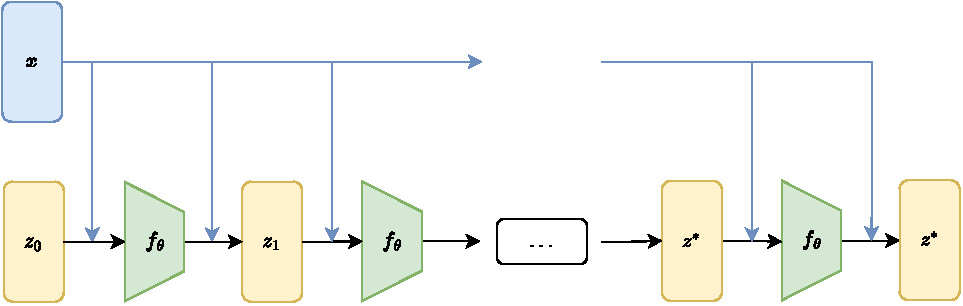
\includegraphics[width=0.9\textwidth]{../figures/deep_equilibrium_models/model_architecture.pdf}
  \caption{\textbf{Discrete DEQ Formulation}: Discrete DEQ Block where the input $x$ is injected at every iteration till the system (with initial state $z_0$) converges to a steady $\zstar$.}
  \label{fig:model_architecture_discrete_deq}
\end{figure}

Deep Equilibrium Networks (DEQs)~\citep{bai_deep_2019} are implicit models where the output space represents a steady-state solution. Intuitively, this represents infinitely deep neural networks with input injection, i.e., an infinite composition of explicit layers $z_{n + 1} = f_\theta(z_n, x)$ with $z_0 = 0$ and $n \rightarrow \infty$. In practice, it is equivalent to evaluating a dynamical system until it reaches a steady state $\zstar = f_\theta(\zstar, x)$.

% \citet{bai_deep_2019, bai_multiscale_2020} perform nonlinear fixed point iterations of the discrete dynamical system using Broyden's method~\citep{broyden1965class, bai_multiscale_2020} to reach this steady-state solution. 

Evaluating DEQs requires solving a steady-state equation involving multiple evaluations of the explicit layer slowing down the forward pass. However, driving the solution to steady-state makes the backward pass very efficient~\citep{johnson2012notes} (See \Cref{sec:sensitivity_analysis_ssproblems}). Despite a potentially infinite number of evaluations of $f_\theta$ in the forward pass, backpropagation only requires solving a linear equation.

\subsection{Nonlinear Solvers}
\label{subsec:nonlinear_solvers_deqs}

In this section, we will exclusively discuss Nonlinear Solvers for solving large steady state problems (i.e., systems with thousands of states).

\subsubsection{Broyden's Method}
\label{subsubsec:broyden_method}

Newton's method is a widely used iterative method for solving nonlinear systems of equations. It is an iterative method that uses the Jacobian matrix to update the solution vector in each iteration.
%
\begin{equation}
  x^{(k+1)} = x^{(k)} - \left( \frac{\partial \func{f}{x^{(k)}}}{\partial x} \right)^{-1} \func{f}{x^{(k)}} \label{eq:newton_method}
\end{equation}
%
However, computing the Jacobian matrix is computationally expensive (cubic time complexity) and memory-wise inefficient. Broyden's method~\citep{broyden1965class} is a quasi-Newton method that approximates the Jacobian matrix using the updates to the solution vector from previous iterations. Specifically, let $f(x)$ be a nonlinear function of the vector $x$, and let $x^{(k)}$ denote the solution vector at the $k$-th iteration. The approximation to the inverse of the Jacobian matrix at iteration $k$ is given by:
%
\begin{equation}
  B^{(k)} = B^{(k-1)} + \left(\frac{\Delta x^{(k)} - B^{(k - 1)} \Delta f^{(k)}}{\Delta x^{(k)^T} B^{(k - 1)} \Delta f^{(k)}}\right) \left(\Delta x^{(k)^T} B^{(k - 1)}\right)
\end{equation}
%
where $\Delta x^{(k)} = x^{(k)} - x^{(k-1)}$ is the step vector, and $\Delta f^{(k)} = \func{f}{x^{(k)}} - \func{f}{x^{(k-1)}}$ is the difference in the function values at the current and previous iterations. $B^{(k-1)}$ is the approximation to the Jacobian matrix at the previous iteration.

The solution vector at the $k$-th iteration is then updated using the following equation:
%
\begin{equation}
  x^{(k+1)} = x^{(k)} - B^{(k)}f(x^{(k)})
\end{equation}
%
Broyden's method has several advantages over Newton's method, including a lower computational cost per iteration, making it feasible for solving large nonlinear system of equations (like deep equilibrium models).

% \subsubsection{Anderson Acceleration}
% \label{subsubsec:anderson_acceleration}

% \todo{verify the equations once}

% Anderson acceleration~\citep{anderson1965iterative} is an iterative method for solving steady state problems of the form $f(x) = x$ that uses a combination of previous iterates to improve the convergence rate of fixed-point iterations. Define the residual $g(x) = f(x) - x$. For notational brevity let, $f^{(k)} =  \func{f}{x^{(k)}}$ and $g^{(k)} = \func{g}{x^{(k)}}$. The basic idea of Anderson acceleration is to construct a sequence $\left\{x^{(0)}, x^{(1)}, x^{(2)}, \ldots, x^{(K)}\right\}$ to accelerate the convergence of a fixed-point sequence. Given an initial guess $x^{(0)}$ and an integer mixing parameter $m \geq 1$, this method performs the following for each iteration $k$:
% %
% \begin{enumerate}
%   \item Compute $m^{(k)} \leftarrow \funct{min}{m, k}$
%   \item Let, $G^{(k)} \leftarrow \left[ g^{(k - m^{(k)})} \ldots g^{(k)} \right]$
%   \item Let, $A^{(k)} \leftarrow \left\{ \alpha = \left( \alpha_0, \ldots, \alpha_{m^{(k)}} \right) \in \mathbb{R}^{m^{(k)} + 1} : \sum_{i = 0}^{m^{(k)}} \alpha_i = 1 \right\}$
%   \item $\alpha^{(k)} \leftarrow \underset{\alpha \in A^{(k)}}{\texttt{argmin}} \left\| G^{(k)} \alpha \right\|_2$
%   \item $x^{(k+1)} \leftarrow \sum_{i = 0}^{m^{(k)}} \alpha^{(k)}_i f^{(k - m^{(k)} + i)}$
% \end{enumerate}
% %
% Anderson acceleration can be very effective for accelerating the convergence of fixed-point iterations for nonlinear problems, especially for problems with slow convergence or oscillatory behavior.

\subsubsection{Limited Memory Broyden's Method}
\label{subsec:limited_memory_broyden}

As described in \Cref{subsubsec:broyden_method}, we can avoid the computational complexity of inverting a Jacobian Matrix by using Broyden's method. However, as pointed out in \citet{bai_multiscale_2020}, even storing the Broyden matrix $B$ for a Nonlinear function $g_\theta: R^{32 \times 32 \times 80} \mapsto R^{32 \times 32 \times 80}$ requires nearly $25GB$ of storage. To circumvent this issue \citet{bai_multiscale_2020} propose a limited memory variant of Broyden's method. The idea is to write the low rank approximation matrix of the inverted jacobian $J^{-1}_{g_\theta}$ ($B$) as the sum of low rank updates:
%
\begin{align}
  B^{(i + 1)}     & = B^{(0)} + \sum_{k = i}^{i + 1} \mathbf{u}^{(k)} \mathbf{v}^{(k)^T} \\
  B^{(i + 1)}     & = B^{(0)} + UV^T                                                     \\
  \texttt{where } & B^{(0)} = -I
\end{align}
%
$\mathbf{u}$ and $\mathbf{v}$ come from Sherman-Morrison Formula~\citep{sherman1950adjustment}. In the limited memory version, \citet{bai_multiscale_2020} store the last $m$ low-rank updates for $\mathbf{u}$ and $\mathbf{v}$, and use a first-in-first-out approach to update $U$ and $V$.

\subsection{Jacobian Free Newton-Krylov Methods (JNFK) for solving Linear Systems}
\label{subsec:newton_krylov_methods}


% \todo{\url{https://en.wikipedia.org/wiki/Generalized_minimal_residual_method}}

% \todo{\url{https://citeseerx.ist.psu.edu/doc/10.1.1.636.3743}}

JFNK Methods are used to solve Linear System of Equations without actually computing the Jacobian Matrix. These methods require the ability to compute matrix-vector products. As we will observe in \Cref{subsec:adjoint_equations_deqs}, ability to avoid the computation of the Jacobian matrix is crucial for large scale steady state problems. JNFK methods use Krylov subspace $K_j$ of dimension $k$ to solve linear equations of the form $A x = b$  where $A \in \mathbb{R}^{n \times n}$ is a sparse, non-symmetric matrix, $b \in \mathbb{R}^n$ is a known vector, and $x \in \mathbb{R}^n$ is the solution vector.
%
\begin{align}
  K_j                 & = \func{\texttt{span}}{r_0, Ar_0, A^2 r_0, \dots, A^{j-1} r_0}\label{eq:krylov_subspace} \\
  \texttt{where } r_0 & = b - A x_0
\end{align}
%
% \todo{chatgpt}
% % In this section, we will describe Generalized Minimal Residual Method (GMRES) a popular JNFK method, that approximates the solution of $Ax = b$ using $x_n \in K_n$ which minimizes the Euclidean norm of the residual $r_n = b - A x_n$.
% The Generalized Minimal Residual Method (GMRES) is a widely used JNFK method for solving large-scale linear systems of equations of the form $Ax=b$. GMRES is an iterative method that generates a sequence of approximate solutions $x_k \in K_k$, where $K_k$ is the Krylov subspace of dimension $k$. GMRES seeks to find the approximate solution $x_k$ that minimizes the Euclidean norm of the residual $r_k = b - Ax_k$ over the subspace $K_k$. Specifically, GMRES solves the minimization problem
% %
% \begin{equation}
%   \min_{x \in K_k} |b - Ax|_2,
% \end{equation}
% %
% where $| \cdot |2$ denotes the Euclidean norm. The solution $x_k$ is obtained using the Arnoldi iteration, which generates an orthogonal basis ${q_1, q_2, \dots, q{k+1}}$ for $K_{k+1}$ using the Arnoldi algorithm. The Arnoldi algorithm constructs the upper Hessenberg matrix $H_k \in \mathbb{R}^{(k+1) \times k}$ and the vector $q_{k+1}$ such that

% \begin{equation}
%   AQ_k = Q_{k+1} H_k,
% \end{equation}

% where $Q_k = [q_1, q_2, \dots, q_k]$ and $Q_{k+1} = [q_1, q_2, \dots, q_{k+1}]$. The solution $x_k$ is then obtained by solving the least-squares problem

% \begin{equation}
%   \min_{y \in \mathbb{R}^k} | \beta e_1 - H_k y |_2,
% \end{equation}

% where $\beta = |b|_2$ and $e_1$ is the first standard basis vector. The approximate solution is then given by

% \begin{equation}
%   x_k = Q_k y_k.
% \end{equation}

% GMRES is known to converge for a wide range of problems and is particularly effective for large-scale, sparse linear systems. However, it may require a large number of iterations to achieve convergence, and each iteration requires solving a linear system, which can be computationally expensive. Additionally, GMRES can be sensitive to the choice of preconditioner, which is used to improve the convergence rate of the algorithm.


\subsection{Adjoint Equations}
\label{subsec:adjoint_equations_deqs}

In \Cref{sec:sensitivity_analysis_ssproblems}, we derived the following linear system of equations:
%
\begin{equation}
  \left( I - \frac{\partial \func{f_\theta}{\zstar}}{\partial \zstar} \right)^T \times \lambda = \left(\frac{\partial \func{g}{\zstar, \theta}}{\partial \zstar}\right)^T
\end{equation}
%
For DEQs, the state space is too large to compute the entire jacobian matrix $\frac{\partial \func{f_\theta}{\zstar}}{\partial \zstar}$. Instead of computing $ A = \left( I - \frac{\partial \func{f_\theta}{\zstar}}{\partial \zstar} \right)^T $, we can use Matrix-Free Methods discussed in \Cref{subsec:newton_krylov_methods} to solve \Cref{eq:ss_lambda_linear}. To use JFNK solvers we need to be efficiently compute:
%
\begin{align}
  A \times \lambda & = \lambda - \left( \frac{\partial \func{f_\theta}{\zstar}}{\partial \zstar} \right)^T  \times \lambda   \\
                   & = \lambda - \left( \lambda^T \times  \frac{\partial \func{f_\theta}{\zstar}}{\partial \zstar} \right)^T
\end{align}
%
The second term is the Vector-Jacobian Product (VJP) which can be efficiently computed by any reverse-mode automatic differentiation framework (without constructing the entire Jacobian). Additionally, in \Cref{eq:ss_total_gradient} we can compute $\lambda^T \times \frac{\partial \func{f_\theta}{\zstar}}{\partial \theta}$ using the VJP trick using any reverse-mode automatic differentiation framework.

% \section{Convergence Criteria}
% \label{sec:ssproblem_convergence_criteria}

% \todo{\url{https://docs.sciml.ai/NonlinearSolve/stable/basics/TerminationCondition/}}

\section{Common Applications of DEQs}
\label{sec:common_applications_deqs}

\section{Accelerating DEQs}
\label{sec:accelerating_deqs}

DEQs share the benefits of implicit neural networks in reducing the memory requirements for training. Specifically, DEQs reduce the memory complexity from $\bigO{SL}$ where $S$ is the dimensions of the output and $L$ is the number of layers to $\bigO{S}$. However, a major concern is the high cost of forward pass which requires solving a steady state problem. An expensive forward pass is not only a bottleneck for training but also hinders deployment, that rely on fast inference. In this section, we discuss some prior works that accelerate the training and inference of DEQs.

\subsection{Jacobian Regularization of DEQs}
\label{subsec:jacobian_regularization_deqs}

\citet{bai2021stabilizing}

\subsection{Jacobian-Free Backpropagation}
\label{subsec:jacobian_free_backpropagation}

\citet{fung2022jfb}

\subsection{Neural Deep Equilibrium Solvers}
\label{subsec:neural_deep_equilibrium_solvers}

\citet{bai2021neural}


% Main Contributions
\part{ACCELERATING NEURAL DIFFERENTIAL EQUATIONS}
\label{part:accelerating_nde}

\chapter[Continuous Deep Equilibrium Networks]{Continuous Deep Equilibrium Networks: Training Neural ODEs Faster by Integrating Them to Infinity}
\label{chapter:infinite_time_neural_odes}

Implicit layer methods, such as Neural ODEs and Deep Equilibrium models~\citep{chen2018neural, bai_deep_2019, ghaoui_implicit_2020}, have gained popularity due to their ability to automatically adapt model depth based on the ``complexity'' of new problems and inputs. The forward pass of these methods involves solving steady-state problems, convex optimization problems, differential equations, etc., all defined by neural networks, which can be expensive. However, training these more generalized models has empirically been shown to take significantly more time than traditional explicit models such as recurrent neural networks and transformers. \textit{Nothing within the problem's structure requires expensive training methods, so we asked, can we reformulate continuous implicit models so that this is not the case}?

\citet{grathwohl2018ffjord, dupont2019augmented, kelly2020learning, finlay2020train} have identified several problems with training implicit networks. These models grow in complexity as training progresses, and a single forward pass can take over 100 iterations~\citep{kelly2020learning} even for simple problems like MNIST. Deep Equilibrium Models~\citep{bai_deep_2019, bai_multiscale_2020} have better scaling in the backward pass but are still bottlenecked by slow steady-state convergence. \citet{bai2021stabilizing} quantified several convergence and stability problems with DEQs. They proposed a regularization technique by exploiting the ``implicitness" of DEQs to stabilize their training. \textit{We marry the idea of faster backward pass for DEQs and continuous modeling from Neural ODEs to create Infinite Time Neural ODEs which scale significantly better in the backward pass and drastically reduce the training time}. % However, such a regularization process is expensive as it requires higher-order automatic differentiation. Their results demonstrated faster prediction times at the expense of greatly increased training times. This leaves an open question as to whether such regularization could be imposed in a cheap or free enough manner to reduce the training cost.

Our main contributions include\footnote{Our code is publicly available at \url{https://github.com/SciML/DeepEquilibriumNetworks.jl}}:
%
\begin{enumerate}
  \item An improved DEQ architecture (Skip-DEQ) that uses an additional neural network to predict better initial conditions.

  \item A regularization scheme (Skip Regularized DEQ) incentivizes the DEQ to learn simpler dynamics and leads to faster training and prediction. Notably, this does not require nested automatic differentiation and thus is considerably less computationally expensive than other published techniques.

  \item A continuous formulation for DEQs as an infinite time neural ODE, which paradoxically accelerates the backward pass over standard neural ODEs by replacing the continuous adjoints with a simple linear system.

  \item We demonstrate the seamless combination of Continuous DEQs with Skip DEQs to create a drop-in replacement for Neural ODEs without incurring a high training cost.
\end{enumerate}
%

The contents of this chapter has appeared in the pre-print: Pal, A., Edelman, A. and Rackauckas, C., 2022. Continuous Deep Equilibrium Models: Training Neural ODEs Faster by Integrating Them to Infinity. arXiv preprint arXiv:2201.12240.~\citep{pal2022mixing}


% \section{Background}
% \label{sec:background}

% Explicit Deep Learning Architectures specify a projection $f: \mathcal{X} \mapsto \mathcal{Z}$ by stacking multiple ``layers". Implicit models, however, define a solution process instead of directly specifying the projection. These methods enforce a constraint on the output space $\mathcal{Z}$ by learning $g: \mathcal{X} \times \mathcal{Z} \mapsto \mathbb{R}^n$. By specifying a solution process, implicit models can effectively vary features like depth to adapt automatically to new scenarios and inputs. Some prominent implicit models include Neural ODEs~\citep{chen2018neural}, where the output $z$ is defined by the ODE $\frac{dz}{dt} = g_\phi(x, t)$. \citet{liu2019neural} generalized this framework to Stochastic Differential Equations (SDEs) by stochastic noise injection, which regularizes the training of Neural ODEs, allowing them to be more robust and achieve better generalization. \citet{bai_deep_2019} designed equilibrium models where the output $z$ was constrained to be a steady state, $z^* = f_\theta(z^*, x)$. Another example of implicit layer architectures is seen in \citet{amos2017optnet, agrawal2019differentiable} set $z$ to be the solution of convex optimization problems.

% Deep Implicit Models essentially removed the design bottleneck of choosing the ``depth" of neural networks. Instead, these models use a ``tolerance" to determine the accuracy to which the constraint needs to be satisfied. Additionally, many of these models only require $O(1)$ memory for backpropagation, thus alluding to potential increased efficiency over their explicit layer counterparts. However, evaluating these models require solving differential equations~\citep{chen2018neural, liu2019neural}, non-linear equations~\citep{bai_deep_2019}, convex optimization problems~\citep{amos2017optnet, agrawal2019differentiable}, etc. Numerous authors~\citep{dupont2019augmented, grathwohl2018ffjord, finlay2020train, kelly2020learning, ghosh2020steer, bai2021stabilizing} have noted that this solution process makes implicit models significantly slower in practice during training and prediction compared to explicit networks achieving similar accuracy.

% \subsection{Neural Ordinary Differential Equations}
% \label{subsec:neural_odes}

% Initial Value Problems (IVPs) are a class of ODEs that involve finding the state at a later time $t_1$, given the value $z_0$ at time $t_0$. \citet{chen2018neural} proposed the Neural ODE framework, which uses neural networks to model the ODE dynamics
% %
% \begin{equation}
%     \frac{dz(t)}{dt} = f_{\theta}\left(z\right)
% \end{equation}
% %
% Using adaptive time stepping allows the model to operate at a variable continuous depth depending on the inputs. Removing the fixed depth constraint of Residual Networks provides a more expressive framework and offers several advantages in problems like density estimation~\cite{grathwohl2018ffjord}, irregularly spaced time series problems~\cite{rubanova2019latent}, etc. Training Neural ODEs using continuous adjoints has the added benefit of constant memory overhead. However, this benefit often leads to slower training since we need to backsolve an ODE. We defer the exact details of the continuous adjoint equations to \citet{chen2018neural}.

% \begin{figure}[t]
%     \centering
%     \includegraphics[width=0.9\linewidth]{images/model_architecture_unified.pdf}
%     \caption{\textbf{Discrete DEQ Formulation}: Discrete DEQ Block where the input $x$ is injected at every iteration till the system (with initial state $z_0$) converges to a steady $z^*$. In Vanilla DEQ, $z_0 = 0$ while in Skip DEQ, an additional explicit model $g_\phi$ (which can potentially share the weights of $f_\theta$) is used to set the initial state $z_0 = g_\phi(x)$.}
%     \label{fig:model_architectures}
% \end{figure}

% \subsection{Deep Equilibrium Models}
% \label{subsec:deep_equilibrium_models}

% Deep Equilibrium Networks (DEQs)~\citep{bai_deep_2019} are implicit models where the output space represents a steady-state solution. Intuitively, this represents infinitely deep neural networks with input injection, i.e., an infinite composition of explicit layers $z_{n + 1} = f_\theta(z_n, x)$ with $z_0 = 0$ and $n \rightarrow \infty$. In practice, it is equivalent to evaluating a dynamical system until it reaches a steady state $z^* = f_\theta(z^*, x)$. \citet{bai_deep_2019, bai_multiscale_2020} perform nonlinear fixed point iterations of the discrete dynamical system using Broyden's method~\citep{broyden1965class, bai_multiscale_2020} to reach this steady-state solution. 

% Evaluating DEQs requires solving a steady-state equation involving multiple evaluations of the explicit layer slowing down the forward pass. However, driving the solution to steady-state makes the backward pass very efficient~\citep{johnson2012notes}. Despite a potentially infinite number of evaluations of $f_\theta$ in the forward pass, backpropagation only requires solving a linear equation.
% %
% % \vspace{-0.5em}
% \begin{gather}
%     z^* = f_\theta(z^*, x)\\
%     \implies \frac{\partial z^*}{\partial \theta} = \frac{f_\theta(z^*, x)}{\partial z^*} \cdot \frac{\partial z^*}{\partial \theta} + \frac{\partial f_\theta(z^*, x)}{\partial \theta}\\
%     \implies \left(I - \frac{\partial f_\theta(z^*, x)}{\partial z^*}\right) \frac{\partial z^*}{\partial \theta} = \frac{\partial f_\theta(z^*, x)}{\partial \theta}
% \end{gather}
% %
% For backpropagation, we need the Vector-Jacobian Product~(VJP):
% %
% \begin{align}
%     \left(\frac{\partial z^*}{\partial \theta}\right)^T v &= \left( \frac{\partial f_\theta(z^*, x)}{\partial \theta} \right)^T\left( I - \frac{\partial f_\theta(z^*, x)}{\partial z^*} \right)^{-T} v\\
%     &= \left( \frac{\partial f_\theta(z^*, x)}{\partial \theta} \right)^T g
% \end{align}
% %
% where $v$ is the gradients from layers after the DEQ module. Computing $\left( I - \frac{\partial f_\theta(z^*, x)}{\partial z^*} \right)^{-T}$ is expensive and makes DEQs non-scalable to high-dimensional problems. Instead, we solve the linear equation $ g =  \left(\frac{\partial f_\theta(z^*, x)}{\partial z^*} \right)^{T} g + v$ using Newton-Krylov Methods like GMRES~\citep{saad1986gmres}. To compute the final VJP, we need to compute $\left( \frac{\partial f_\theta(z^*, x)}{\partial \theta} \right)^T g$, which allows us to efficiently perform the backpropagation without explicitly computing the Jacobian.

% \subsubsection{Multiscale Deep Equilibrium Network}
% \label{subsubsec:mdeq}

% Multiscale modeling~\citep{burt1987laplacian} has been the central theme for several deep computer vision applications~\citep{farabet2012learning, yu2015multi, chen2016attention, chen2017deeplab}. The standard DEQ formulation drives a single feature vector to a steady state. \citet{bai_multiscale_2020} proposed Multiscale DEQ (MDEQ) to learn coarse and fine-grained feature representations simultaneously. MDEQs operate at multiple feature scales $z = \left\{ z_1, z_2, \dots, z_n \right\}$, with the new equilibrium state $z^* = f_\theta(z_1^*, z_2^*, \dots, z_n^*, x)$. All the feature vectors in an MDEQ are interdependent and are simultaneously driven to a steady state. \citet{bai_multiscale_2020} used a Limited-Memory Broyden Solver~\citep{broyden1965class} to solve these large scale computer vision problems. We use this MDEQ formulation for all our classification experiments.

% \subsubsection{Jacobian Stabilization}
% \label{subsubsec:jacobian_stabilization}

% Infinite composition of a function $f_\theta$ does not necessarily lead to a steady-state -- chaos, periodicity, divergence, etc., are other possible asymptotic behaviors. The Jacobian Matrix $J_{f_\theta}(z^*)$ controls the existence of a stable steady-state and influences the convergence of DEQs in the forward and backward passes. \citet{bai2021stabilizing} describes how controlling the spectral radius of $J_{f_\theta}(z^*)$ would prevent simpler iterative solvers from diverging or oscillating. \citet{bai2021stabilizing} introduce a Jacobian term to the training objective to regularize the model training. The authors use the Hutchinson estimator~\citep{hutchinson1989stochastic} to compute and regularize the Frobenius norm of the Jacobian.
% %
% \begin{equation}
%     \mathcal{L}_{jac} = \lambda_{jac} \frac{\| \epsilon^T J_{f_\theta}(z^*) \|_2^2}{d}; \quad \epsilon \sim \mathcal{N}(0, I_d)
% \end{equation}
% %
% While well-motivated, the disadvantage of this method is that the Hutchinson trace estimator requires automatic differentiation in the loss function, thus requiring higher order differentiation in the training process and greatly increasing the training costs. However, in return for the increased cost, it was demonstrated that increased robustness followed, along with faster forward passes in the trained results. Our methods are orthogonal to the Jacobian stabilization process. In \Cref{sec:experiments}, we provide empirical evidence on composing our models with Jacobian Stabilization to achieve even more robust results.

% \section{Methods}
% \label{sec:methods}

\section{Continuous Deep Equilibrium Networks}
\label{sec:continuous_deqs}

Deep Equilibrium Models have traditionally been formulated as steady-state problems for a discrete dynamical system. However, discrete dynamical systems come with a variety of shortcomings. Consider the following linear discrete dynamical system (See \Cref{fig:linear_discrete_dynamical_system}):
%
\begin{align}
    u_{n + 1} &= \alpha \cdot u_n \\
    \texttt{ where } \|\alpha\| &< 1 \texttt{ and } u_0 = 1
\end{align}
%
This system converges to a steady state of $u_\infty = 0$. However, in many cases, this convergence can be relatively slow. If $\alpha = 0.9$, then after 10 steps, the value is $u_{10} = 0.35$ because a small amount only reduces each successive step. Thus convergence could only be accelerated by taking many steps together. Even further, if $\alpha = -0.9$, the value ping-pongs over the steady state $u_{1} = -0.9$, meaning that if we could take some fractional step $u_{\delta t}$ then it would be possible to approach the steady state much faster.

% \begin{figure}[H]
%     % Remove if space-constrained
%     \centering
%     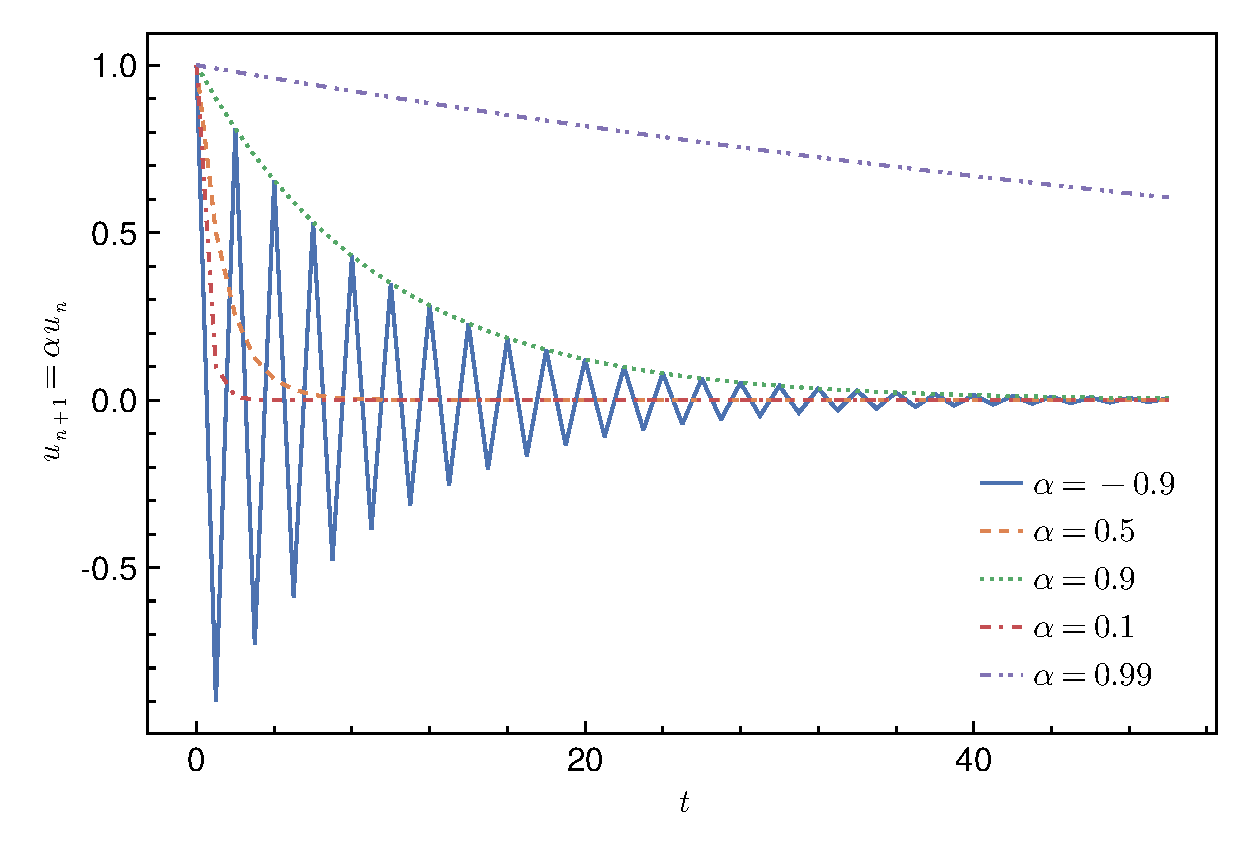
\includegraphics[width=0.5\linewidth]{images/linear_discrete_dynamical_system}
%     \caption{\textbf{Slow Convergence of Simple Linear Discrete Dynamical Systems}}
%     \label{fig:linear_discrete_dynamical_system}
% \end{figure}

\citet{rico1992discrete, bulsari1995neural} describe several other shortcomings of using discrete steady-state dynamics over continuous steady-state dynamics. These issues combined motivate changing from a discrete description of the system (the fixed point or Broyden's method approach) to a continuous description of the system that allows adaptivity to change the stepping behavior and accelerate convergence.

To this end, we propose an alternate formulation for DEQs by modeling a continuous dynamical system (Continuous DEQ) where the forward pass is represented by an ODE which is solved from $t_0 = 0$ to $t_1 = \infty$:
%
\begin{equation}
    \frac{dz}{dt} = \func{f_\theta}{z, x} - z
\end{equation}
%
where $f_\theta$ is an explicit neural network. Continuous DEQs leverage fast adaptive ODE solvers, which terminate automatically once the solution is close to a steady state, i.e., $\frac{dz^*}{dt} = 0$, which then satisfies $\func{f_\theta}{z^*, x} = z^*$ and is thus the solution to the same implicit system as before.

The Continuous DEQ can be considered an infinite-time neural ODE in this form. However, almost paradoxically, the infinite time version is cheaper to train than the finite time version as its solution is the solution to the nonlinear system, meaning the same implicit differentiation formula of the original DEQ holds for the derivative. This means that no backpropagation through the steps is required for the Continuous DEQ, and only a linear system must be solved. In \Cref{sec:experiments}, we empirically demonstrate that Continuous DEQs outperform Neural ODEs in terms of training time while achieving similar accuracies.

% Indeed, the robustness of the DEQ is even improved through this process because, in practice, the maximum iterations of the DEQ are bound~\citep{bai_deep_2019, bai_multiscale_2020, bai2021stabilizing}. DEQs often do not converge to a steady state due to this bound. In \Cref{sec:experiments}, we observe that for small-scale problems Skip~DEQs improve convergence to steady state  even where a DEQ fails due to its increased convergence speed. However, this behavior fades away once we move to the higher parameter count regime. When combining Skip~DEQs % This ability allows Skip DEQs to be trained with a more stable gradient signal since the adjoint equation assumes steady-state convergence during the forward pass.

\section{Skip Deep Equilibrium Networks}
\label{sec:skip_deqs}

\citet{bai_deep_2019, bai_multiscale_2020} set the initial condition $u_0 = 0$ while solving a DEQ. Assuming the existence of a steady state, the solvers will converge given enough iterations. However, each iteration is expensive, and a poor guess of the initial condition makes the convergence slower. To counteract these issues, we introduce an alternate architecture for DEQ (Skip~DEQ), where we use an explicit model $g_\phi$ to predict the initial condition for the steady-state problem $u_0 = g_\phi(x)$\footnote{We note that the concurrent work \citet{bai2021neural} introduced a similar formulation as a part of HyperDEQ}. We jointly optimize for $\left\{\theta, \phi\right\}$ by adding an auxiliary loss function:
%
\begin{equation}
    \mathcal{L}_{\texttt{skip}} = \lambda_{\texttt{skip}} \cdot \| f_\theta(z^*, x) - g_\phi(x) \|
\end{equation}
%
Intuitively, our explicit model $g_\phi$ better predicts a value closer to the steady-state (over the training iterations), and hence we need to perform fewer iterations during the forward pass. Given that its prediction is relatively free compared to the cost of the DEQ, this technique could decrease the cost of the DEQ by reducing the total number of iterations required. However, this prediction-correction approach still uses the result of the DEQ for its final predictions and thus should achieve robustness properties equal.

\section{Skip Regularized DEQ: Regularization Scheme without Extra Parameters}
\label{sec:skip_reg_deq}

One of the primary benefits of DEQs is the low memory footprint of these models. Introducing an explicit model $g_\phi$ increases the memory requirements for training. To alleviate this problem, we propose a regularization term to minimize the L1 distance between the first prediction of $f_\theta$ and the steady-state solution:
%
\begin{align}
    \mathcal{L}_{\texttt{skip\_reg}} = \lambda_{\texttt{skip}} \cdot \| f_\theta(z^*, x) - f_\theta(0, x) \|
\end{align}
%
This technique follows the same principle as the Skip DEQ where the DEQ's internal neural network is now treated as the prediction model. We hypothesize that this introduces an inductive bias in the model to learn simpler training dynamics.

\chapter{Opening the Blackbox: Global Regularization using Local Error \& Stiffness Estimates}
\label{chapter:internal_solver_heuristics_regularized_neural_des}

How many hidden layers should you choose in your recurrent neural network? \citet{chen2018neural} showed that the answer could be found automatically by using a continuous reformulation, the neural ordinary differential equation, and allowing an adaptive ODE solver to effectively choose the number of steps to take. Since then the idea was generalized to other domains such as stochastic differential equations \citep{liu2019neural, rackauckas2020universal} but one fact remained: \textit{solving a neural differential equation is expensive, \& training a neural differential equation is even more so}.

In this thesis, we present a generally applicable method to force the neural differential equation training process to choose the least expensive option. We open the blackbox and show how using the numerical heuristics baked inside of these sophisticated differential equation solver codes allows for identifying the cheapest equations without requiring extra computation. However, ``opening the blackbox'' has several downsides -- they are \textit{harder to integrate into existing code-bases} and are \textit{more memory intensive}. Hence, we describe methods that exploit random sampling to leverage the benefits of ``opening the blackbox'' without actually requiring specialized training methods and the associated memory overhead.

The contents of this chapter has appeared previously in the publication: Pal, A., Ma, Y., Shah, V. and Rackauckas, C.V., 2021, July. Opening the Blackbox: Accelerating Neural Differential Equations by Regularizing Internal Solver Heuristics. In International Conference on Machine Learning (pp. 8325-8335). PMLR. \citep{pal2021opening}


\section{Opening the Blackbox: Global Regularization using Local Error \& Stiffness Estimates}
\label{sec:global_regularization_using_local_error_and_stiffness_estimates}

\Cref{sec:adaptive_time_stepping} describes how larger local error estimates $\eest$ lead to reduced step sizes and thus a higher overall cost in the neural ODE training and predictions. Given this, we propose regularizing the neural ODE training process by the total local error in order to learn neural ODEs with as large step sizes as possible. Thus we define the regularizing term:
%
\begin{equation}
  \label{eq:reg_eest_global}
  \left(\mathcal{R}_{E}\right)_g = \sum_j \left(\eest\right)_j \cdot |\dt_j|
\end{equation}
%
summing over $j$ the time steps of the solution. This was done by accumulating the $\left(\eest\right)_j$ from the internals of the time stepping process at the end of each step. We note that this is similar to the regularization proposed in \citet{kelly2020learning}, namely:
%
\begin{equation}
  \label{eq:reg_global_kelly}
  \left(\mathcal{R}_{K}\right)_g = \int_{t_0}^{t_1} \left\|\frac{d^K z(t)}{dt^K}\right\| \dt
\end{equation}
%
where integrating over the $K^{th}$ derivatives is proportional to the principle (largest) truncation error term of the Runge-Kutta method~\citep{hairer1}. However, this formulation requires high order automatic differentiation (which then is layered with reverse-mode automatic differentiation) which can be an expensive computation~\citep{zhang2008computing} while \Cref{eq:reg_eest_global} requires no differentiation.

Similarly, the stiffness estimates (\Cref{sec:automatic_stiffness_detection}) at each step can be summed as:
%
\begin{equation}
  \label{eq:reg_stiffness_global}
  \left(\mathcal{R}_{S}\right)_g = \sum_j \left(\sest\right)_j \cdot |\dt_j|
\end{equation}
%
giving a computational heuristic for the total stiffness of the equation. Notably, both of these estimates $\left(\eest\right)_j$ and $\left(\sest\right)_j$ are already computed during the course of a standard explicit Runge-Kutta solution, making the forward pass calculation of the regularization term computationally free.


\section{Adjoints of Internal Solver Heuristics}
\label{sec:adjoints_of_internal_solver_heuristics}

Notice that $\left(\eest\right)_j = \sum_{i = 1}^s \left(b_i - \tilde{b_i}\right) \cdot k_i$ cannot be constructed directly from the $\func{z}{t_j}$ trajectory of the ODE's solution. More precisely, the $k_i$ terms are not defined by the continuous ODE but instead by the chosen steps of the solver method. Continuous adjoint methods for neural ODEs~\citep{chen2018neural, zhuang2021mali} only define derivatives in terms of the ODE quantities. This is required in order exploit properties such as allowing different steps in reverse and reversibility for reduced memory, and in constructing solvers requiring fewer NFEs~\citep{kidger2020hey}. Indeed, computing the adjoint of each stage variable $k_i$ can be done, but is known as discrete sensitivity analysis and is known to be equivalent to automatic differentiation of the solver~\citep{zhang2014fatode}. Thus to calculate the derivative of the solution simultaneously to the derivatives of the solver states, we used direct automatic differentiation of the differential equation solvers for performing the experiments~\citep{innes2018don}. We note that discrete adjoints are known to be more stable than continuous adjoints~\citep{zhang2014fatode} and in the context of neural ODEs have been shown to stabilize the training process leading to better fits \citep{gholami2019anode,onken2020discretize}. While more memory intensive than some forms of the continuous adjoint, we note that checkpointing methods can be used to reduce the peak memory \citep{dauvergne2006data}. We note that this is equivalent to backpropagation of a fixed time step discretization if the step sizes are chosen in advance, and verify in the example code that no additional overhead is introduced.


\section{Experimental Results for Global Regularization}
\label{sec:experimental_results_global_regularized_neural_des}


\section{Discussion on Global Regularization of Neural DEs}
\label{sec:discussion_on_global_regularization_of_neural_des}

Numerical analysis has had over a century of theoretical developments leading to efficient adaptive methods for solving many common nonlinear equations such as differential equations. Here we demonstrate that by using the knowledge embedded within the heuristics of these methods we can accelerate the training process of neural ODEs.

We note that on the larger sized PhysioNet and MNIST examples we saw significant speedups while on the smaller differential equation examples we saw only minor performance improvements. This showcases how the NFE becomes a better estimate of the total compute time as the cost of the ODE $f$ (and SDE $g$) increase when the model size increases.

This result motivates efforts in differentiable programming~\citep{wang2018backpropagation, abadi2019simple, rackauckas2020generalized} which enables direct differentiation of solvers since utilizing the solver's heuristics may be crucial in the development of advanced techniques. This idea could be straightforwardly extended not only to other forms of differential equations, but also to other ``implicit layer'' machine learning methods. For example, Deep Equilibrium Models (DEQ)~\citep{bai_deep_2019} model the system as the solution to an implicit function via a nonlinear solver like Bryoden or Newton's method. Heuristics like the ratio of the residuals have commonly been used as a convergence criterion and as a work estimate for the difficulty of solving a particular nonlinear equation~\citep{wanner1996solving}, and thus could similarly be used to regularize for learning DEQs whose forward passes are faster to solve. Similarly, optimization techniques such as BFGS~\citep{kelley1999iterative} contain internal estimates of the Hessian which can be used to regularize the stiffness of ``optimization as layers'' machine learning architectures like OptNet~\citep{amos2017optnet}. However, in these cases we note that continuous adjoint techniques have a significant computational advantage over discrete adjoint methods because the continuous adjoint method can be computed directly at the point of the solution while discrete adjoints would require differentiating through the iteration process. Thus while a similar regularization would exist in these contexts, in the case of differential equations the continuous and discrete adjoints share the same computational complexity which is not the case in methods which iterate to convergence. Further study of these applications would be required in order to ascertain the effectiveness in accelerating the training process, though by extrapolation one may guess that at least the forward pass would be accelerated.

\subsection{Limitations of Global Regularization using Error and Stiffness Estimates}
\label{subsec:limitations_of_using_error_and_stiffness_estimates}

While these experiments have demonstrated major performance improvements, it is pertinent to point out the limitations of the method. One major point to note is that this only applies to learning neural ODEs for maps $z(0) \mapsto z(1)$ as is used in machine learning applications of the architecture~\citep{chen2018neural}. Indeed, a neural ODE as an ``implicit layer'' for predictions in machine learning does not require identification of dynamical mechanisms. However, if the purpose is to learn the true governing dynamics a physical system from timeseries data, this form of regularization would bias the result, dampening higher frequency responses leading to an incorrect system identification. Approaches which embed neural networks into solvers could be used in such cases~\citep{shen2020deep,poli2020hypersolvers}. Indeed we note that such Hypereuler approaches could be combined with the ERNODE regularization on machine learning prediction problems, which could be a fruitful avenue of research. Lastly, we note that while either the local error and stiffness regularization was effective on each chosen equation, neither was effective on all equations and at this time there does not seem to be a clear a priori indicator as to which regularization is necessary for a given problem. While it seems the error regularization was more effective on the image classification tasks while the stiffness regularization was more effective on the time series task, we believe more experiments will be required in order to ascertain whether this is a common phenomena, possibly worthy of theoretical investigation.

\chapter{Closing the Blackbox: Local Regularization of Neural DEs using Local Error Estimates}
\label{chapter:local_regularization_neural_odes}

Implicit Models, such as Neural Ordinary Differential Equations~\cite{chen2018neural} and Deep Equilibrium Models~\cite{bai_deep_2019, pal2022mixing}, have emerged as a promising technique to determine the depth of neural networks automatically. To maximize performance on a dataset, explicit models are tuned to the ``hardest'' training sample, which hurts the inference timings for ``easier'' -- more abundant -- samples. Using adaptive differential equation solvers allow these implicit models to choose the number of steps they need effectively. This idea of representing neural networks as ODEs has since been generalized to Stochastic Differential Equations~\citep{liu2019neural, rackauckas2020universal} and other architectures to improve robustness.

Despite the rapid progress in these methods, the core problem of the scalability of these models is still persistent. Several solutions to these have been proposed:
%
\begin{itemize}
  \item \citet{kelly2020learning, finlay2020train} use higher order derivatives for regularization.
  \item \citet{poli2020hypersolvers} learn neural solvers to solve Neural ODEs faster.
  \item In \Cref{chapter:internal_solver_heuristics_regularized_neural_des}, we described a ``zero-cost'' global regularization scheme.
  \item \citet{ghosh2020steer} randomize the integration stop time to ``smoothen'' the dynamics.
\end{itemize}
%
All these methods have definite tradeoffs. \citet{finlay2020train, kelly2020learning} have relied on using higher-order regularization terms to constrain the space of learnable dynamics. These models speed up predictions, but their benefits are often overshadowed by a massive training slowdown~\citep{pal2021opening}. More recently, quite a few first-order schemes have been proposed. \citet{ghosh2020steer} randomized the endpoint of Neural ODEs to incentivize simpler dynamics. However, \citet{pal2021opening} didn't find significant benefits of using STEER in their experiments. \citet{pal2021opening} used internal solver heuristics -- local error and stiffness estimates -- to control the learned dynamics in a way that decreased both prediction and training time.

This paper presents a generally applicable method to force the neural differential equation training process to choose the least expensive option. We build upon the global regularization scheme proposed in \citet{pal2021opening} and ``close'' the blackbox allowing our method to work across various sensitivity algorithms. Our main contributions include the following\footnote{Our code is publicly available at \url{https://github.com/avik-pal/LocalRegNeuralDE.jl}}:
%
\begin{enumerate}
  \item We show that our local regularization method -- building upon the primitives proposed in \citet{pal2021opening} -- performs at par with global regularization.

  \item We present two sampling methods that trade-off small computational costs for consistently better performance.

  \item Using local regularization allows our models to leverage optimize-then-discretize in the backward pass (in addition to discretize-then-optimize methods). Our method works around the several engineering limitations of automatic differentiation (AD) systems~\citep{rackauckas_2022} that are needed to make global regularization work.

  \item We empirically show that regularizing solver heuristics with biased sampling stabilizes the training of larger neural ODEs.
\end{enumerate}
%

The contents of this chapter has appeared previously in the publication: Pal, A., Edelman, A. and Rackauckas, C., 2023. Locally Regularized Neural Differential Equations: Some Black Boxes Were Meant to Remain Closed!. In International Conference of Machine Learning. PMLR. \citep{pal2023locally}

\begin{figure}[t]
  \centering
  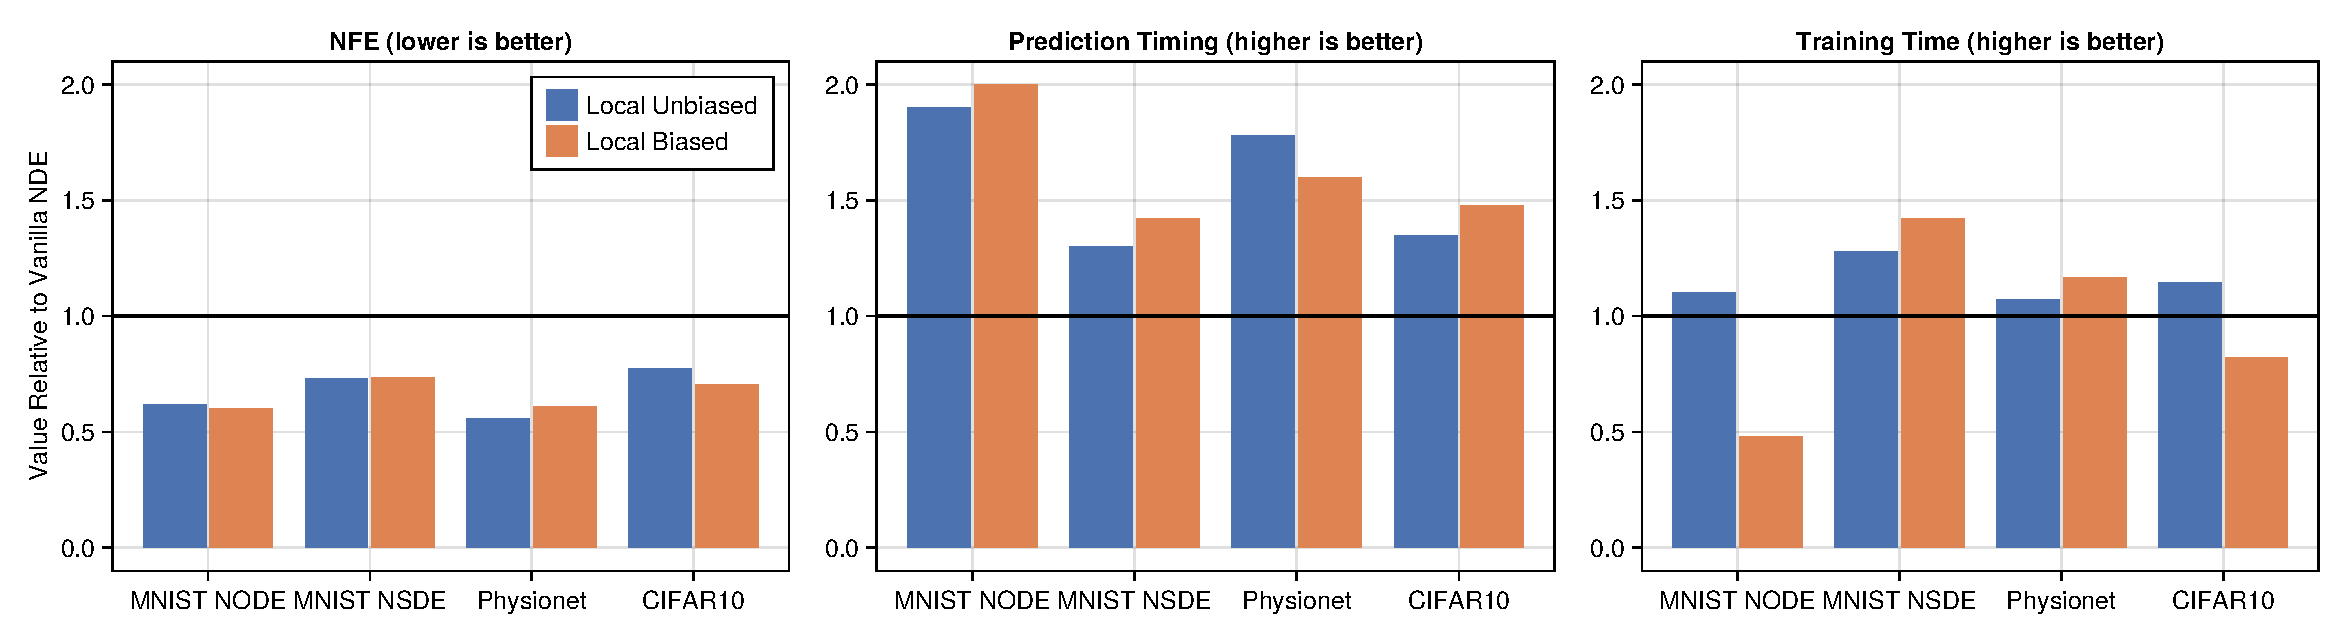
\includegraphics[width=\textwidth]{../figures/local_regularizing_neural_des/summary_plot.pdf}
  \caption{\textbf{Locally Regularized NDE leads to faster predictions and faster training compared to vanilla NDE.}}
  \label{fig:localreg_summary_plot}
\end{figure}


\section{Randomized Local Regularization: Overcoming the shortcomings of Global Regularization}
\label{sec:randomized_local_regularization_overcoming_the_shortcomings_of_global_regularization}


In \Cref{subsec:limitations_of_using_error_and_stiffness_estimates}, we discussed the downsides of using global regularization with local error estimates. To summarize:
%
\begin{enumerate}
  \item Global Regularization relies on discrete sensitivity analysis, which is \textit{more memory intensive}.

  \item Global Regularization depends on AD tooling to support dynamic compute graphs in an efficient way, making it \textit{hard to incorporate into existing code-bases}.
\end{enumerate}
%
To get around these limitations, we developed a new technique using local sampling of error estimates at specific time points, rather than globally over the full interval. We deal with sampling the ``appropriate'' time point for regularization by two strategies:
%
\begin{itemize}
  \item \textbf{\Cref{alg:local_regularization_unbiased_sampling} Unbiased Sampling}: We random uniformly sample the time-point in the integration time span. Intuitively, since we will perform the training for ``a large number of steps,'' the learned dynamical system would end up being faster to solve ``everywhere'' over the time span.

  \item \textbf{\Cref{alg:local_regularization_biased_sampling} Biased Sampling}: Adaptive Time-Stepping Differential Equation Solvers naturally take more steps around the area, which is harder to integrate. We can bias the regularization to operate around parts of the dynamical system which are ``harder'' by sampling a time-point from the solution time points.
\end{itemize}
%

\begin{algorithm}[t]
  \caption{\textbf{Unbiased Sampling: Training}}
  \label{alg:local_regularization_unbiased_sampling}
  \begin{algorithmic}[1]
    \Function{$\texttt{ERNODE}_{\texttt{Unbiased}}$}{$x$, $f_\theta$, $t_{\texttt{span}}$}
    \State \texttt{Define} $\frac{du}{dt} = f_\theta(u, t)$
    \State $t_0, t_1 \gets t_{span}$
    \State $\treg \sim \mathbb{U}\left[t_0,~t_1\right]$
    \State $\texttt{sol} \gets \texttt{solve}(\frac{du}{dt}, \texttt{ DE Solver},~t_{\texttt{span}})$
    \State $u_{\treg} \gets \texttt{sol}(\treg)$
    \State Run single step for the solver with time-span $(\treg, t_1)$
    \State $\texttt{r} \gets $ Local Error Estimate $@ t=\treg$
    \State \Return{$\texttt{sol}, \texttt{r}$}
    \EndFunction
  \end{algorithmic}
\end{algorithm}

\subsection{Unbiased Sampling of Local Error Estimates}
\label{subsec:unbiased_sampling_of_local_error_estimates}

When training a Neural ODE, the integration time-span is fixed. Training any deep learning model involves several thousand steps. We compute the total local error estimate over the entire time-span when performing global regularization. For unbiased sampling, we hypothesize that if we regularize at random uniformly sampled time points in the time-span, the learned dynamical system will demonstrate similar properties in terms of NFE compared to global regularization. Our new regularization term becomes $\left(\mathcal{R}_{E}\right)_{\texttt{unbiased}}$ as:
%
\begin{gather}
  \left(\mathcal{R}_{E}\right)_{\texttt{unbiased}} = \left(\texttt{E}_{\texttt{Est}}\right)_{\treg} \cdot |\dt_{\treg}|\\
  \treg \sim \mathbb{U}[\texttt{tspan}]
\end{gather}
%

\begin{algorithm}[t]
  \caption{\textbf{Biased Sampling: Training}}
  \label{alg:local_regularization_biased_sampling}
  \begin{algorithmic}[1]
    \Function{$\texttt{ERNODE}_{\texttt{Biased}}$}{$x$, $f_\theta$, $t_{\texttt{span}}$}
    \State \texttt{Define} $\frac{du}{dt} = f_\theta(u, t)$
    \State $t_0, t_1 \gets t_{span}$
    \State $\texttt{sol} \gets \texttt{solve}(\frac{du}{dt}, \texttt{ DE Solver},~t_{\texttt{span}})$
    \State $\treg \sim \mathbb{U}\left(\texttt{sol}.t\right)$
    \State $u_{\treg} \gets \texttt{sol}(\treg)$
    \State Run single step for the solver with time-span $(\treg, t_1)$
    \State $\texttt{r} \gets $ Local Error Estimate $@ t=\treg$
    \State \Return{$\texttt{sol}, \texttt{r}$}
    \EndFunction
  \end{algorithmic}
\end{algorithm}

\subsection{Biased Sampling of Local Error Estimates}
\label{subsec:biased_sampling_of_local_error_estimates}

\begin{wrapfigure}{r}{0.5\linewidth}
  \centering
  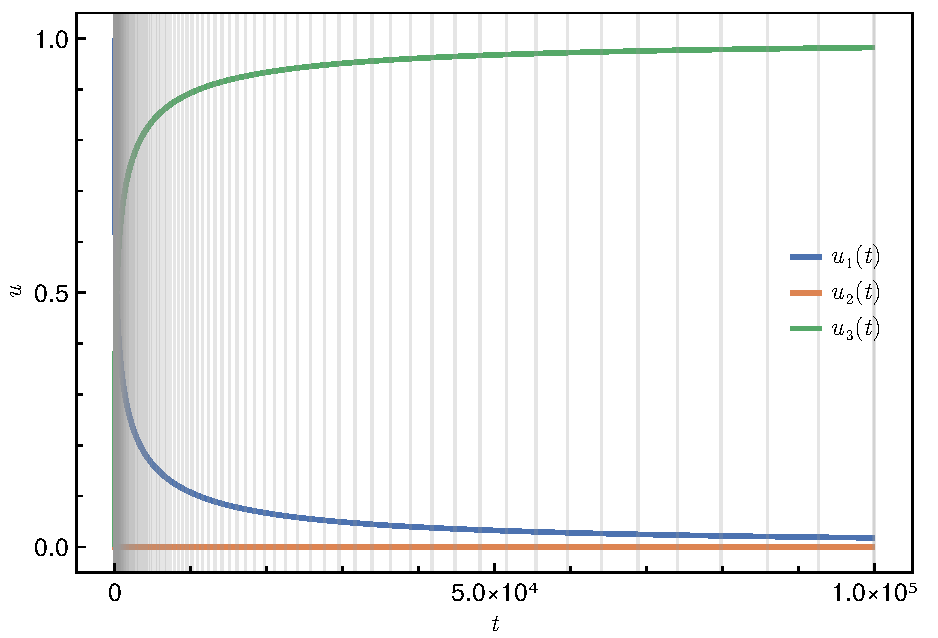
\includegraphics[width=0.95\linewidth]{../figures/local_regularizing_neural_des/biased_sampling_robertson_example}
  \captionof{figure}{\textbf{Robertson Stiff ODE System}: Solving stiff systems like Robertson~\citep{robertson1966solution} (using Rodas5~\citep{piche1995stable}) involves spending around $75\%$ of the time in $t < 5000$ (i.e. $5\%$ of the time-span). The vertical lines denote the time-points at which the ODE System was solved.}
  \label{fig:robertson_stiff_system}
\end{wrapfigure}


Consider a simple scenario where the learned dynamics of the DE is harder to solve in $\left[0.25, 0.35\right]$, and we are solving the DE from $t_0 = 0$ to $t_1 = 1$. Our primary aim is to modify the learned system s.t. it becomes simpler to solve in $\left[0.25, 0.35\right]$. If we use unbiased sampling, the probability that we regularize at $\treg \in \left[0.25, 0.35\right]$ is $0.1$ (which is low). The problem gets even more severe if the range is lowered. An extreme version of this problem is observed for stiff systems like Robertson's Equations~(See \Cref{fig:robertson_stiff_system}) where $75\%$ of the time is spent in solving $5\%$ of the problem. We note that these extreme scenarios rarely occur for traditional deep learning tasks since \citet{pal2021opening} observed minor speedups using stiffness regularization. However, the problem that some parts of the dynamical system are harder to integrate persists, and designing a regularization scheme targeting those parts is highly desirable.

We considered a simple scenario where the learned dynamical system was fixed. However, while training NDEs, this system evolves with training, and apriori predicting the more difficult portions to integrate is not feasible. Adaptive solvers take more frequent steps in the parts of the DE where it is harder to integrate. \citet{anantharaman2020accelerating} leveraged this property of adaptive solvers to learn surrogates for stiff systems. Since these solvers adapt to concentrate around the most numerically difficult time points, we automatically obtain the time points where we want to regularize the model. Hence, for our biased sampling regularize, we uniformly sample the regularization timepoint $\treg$ from the time points at which the solver solved the differential equation.

\begin{table}[t]
  \centering
  \adjustbox{max width=\textwidth}{
    \centering
    \begin{tabular}{lcc}
      \toprule
      \thead{Sensitivity Algorithm}                                          & \thead{Memory Requirement}                 & \thead{Memory Requirement with Local Reularization}         \\
      \midrule
      Backsolve Adjoint \citep{chen2018neural}                               & $\bigO{s}$                                 & $\bigO{s \times (1 + \mathrm{stages})}$                                \\
      Backsolve Adjoint with Checkpointing \citep{chen2018neural}            & $\bigO{s \times c}$                        & $\bigO{s \times (c  + \mathrm{stages})}$                      \\
      Interpolating Adjoint \citep{hindmarsh2005sundials}                    & $\bigO{s \times t}$                        & $\bigO{s \times (t  + \mathrm{stages})}$                      \\
      Interpolating Adjoint with Checkpointing \citep{hindmarsh2005sundials} & $\bigO{s \times c}$                        & $\bigO{s \times (c + \times \mathrm{stages})}$                       \\
      Quadrature Adjoint \citep{kim2021stiff}                                & $\bigO{\left(s + p\right) \times t}$       & $\bigO{\left(s + p\right) \times t + s \times \mathrm{stages}}$      \\
      Direct Reverse Mode Differentiation                                    & $\bigO{s \times t \times \mathrm{stages}}$ & $\bigO{s \times \left(t + 1\right) \times \mathrm{stages}}$ \\
      \bottomrule
    \end{tabular}
  }
  \caption{\textbf{Memory Requirements for various Sensitivity Algorithms for ODEs with Local Regularization}}
  \label{tab:memory_requirements_sensitivity_analysis_odes_with_local_reg}
\end{table}

\section{Adjoint for Local Regularized Neural Differential Equations}
\label{sec:adjoint_for_local_regularized_neural_differential_equations}

Adjoint Sensitivity Analysis of Local Regularization works by piggy-backing on the existing adjoint sensitivity analysis algorithms. Our algorithm is effectively equivalent to using the default adjoint sensitivity algorithm with direct reverse mode differentiation through a single step of the solver, i.e. $ t = 1$. Thus, our algorithm adds a constant overhead of $\bigO{s \times \mathrm{stages}}$ memory to the underlying sensitivity algorithm.

\section{Experimental Results}
\label{sec:experimental_results_local_regularized_neural_des}

In this section, we compare the effectiveness of unbiased and biased local regularization's effectiveness on the training and prediction timings of NDEs. We choose image classification and time series prediction problems in line with prior works on accelerating NDEs. We consider the following baselines:
%
\begin{enumerate}
  \item Vanilla Neural ODE with Continuous Interpolating Adjoint.

  \item Vanilla Neural SDE with discrete sensitivities.

  \item Global Regularization of Neural Differential Equations using discrete sensitivity analysis \citep{pal2021opening}.

  \item TayNODE~\citep{kelly2020learning} and STEER~\citep{ghosh2020steer} for models reported in \citet{pal2021opening}.
\end{enumerate}
%

We use the DifferentialEquations.jl~\citep{rackauckas2019diffeqflux} and Lux.jl~\citep{pal2022lux} software stack written in the Julia Programming Language~\citep{Julia-2017} for all our experiments.

Some details about the data presented in the tables:
%
\begin{itemize}
  \item All experimental results in the tables marked with \textparagraph~ were taken directly from \citet{pal2021opening}.

  \item We have tried to match the hardware details presented in the paper and the corresponding GitHub repository for \citet{pal2021opening}, but we note that differences in wall clock timings can be partially attributed to hardware.

  \item TayNODE~\citep{kelly2020learning} uses a different ODE integrator. Hence the NFEs are not directly comparable.
\end{itemize}
%

\begin{figure}[t]
  \centering
  \begin{minipage}[c]{0.49\textwidth}
    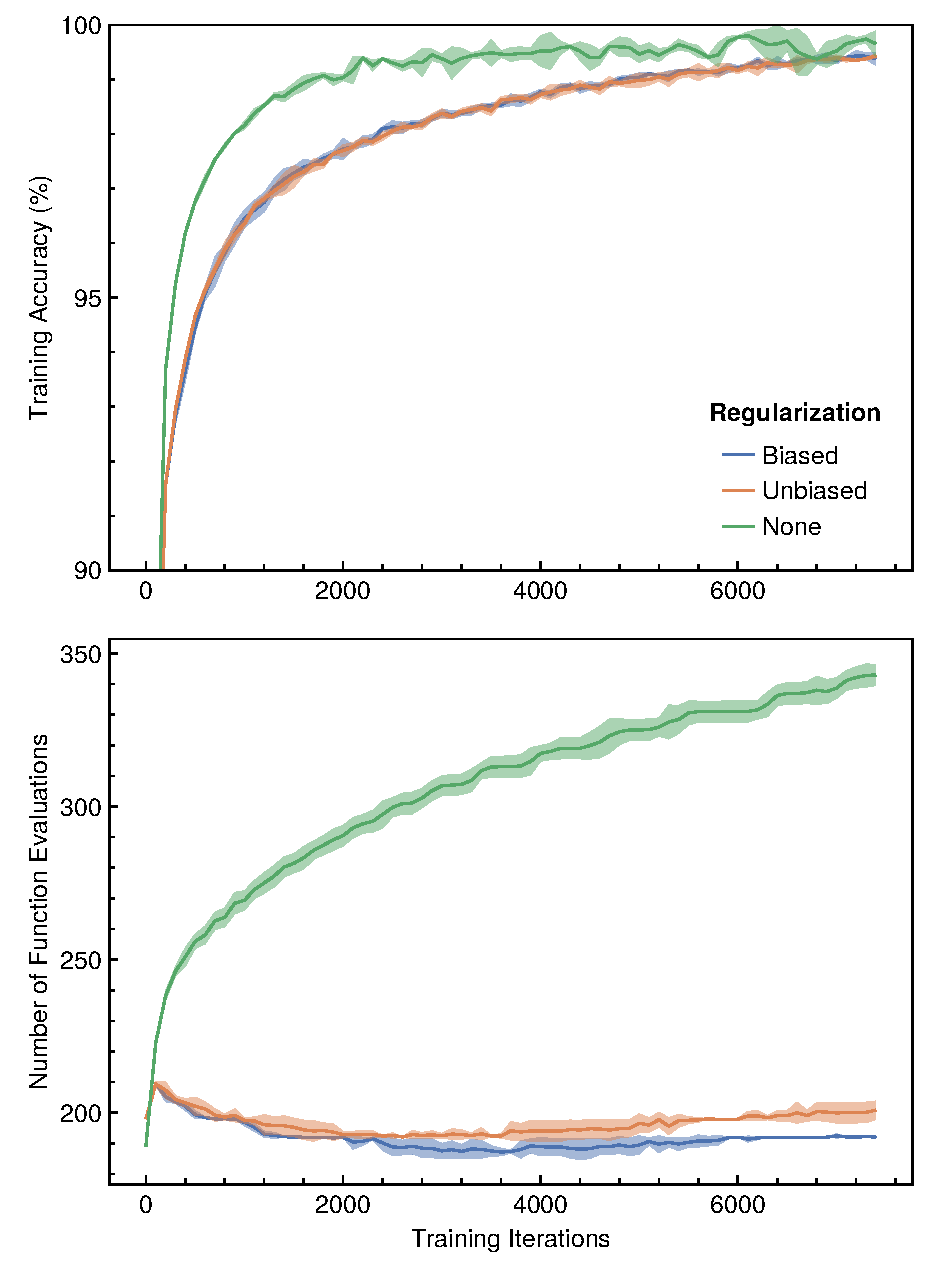
\includegraphics[width=\linewidth]{../figures/local_regularizing_neural_des/mnist_ode.pdf}
    \caption{\textbf{MNIST Classification using Neural ODE}}
    \label{fig:mnist_node_localreg}
  \end{minipage}
  \hfill
  \begin{minipage}[c]{0.49\textwidth}
    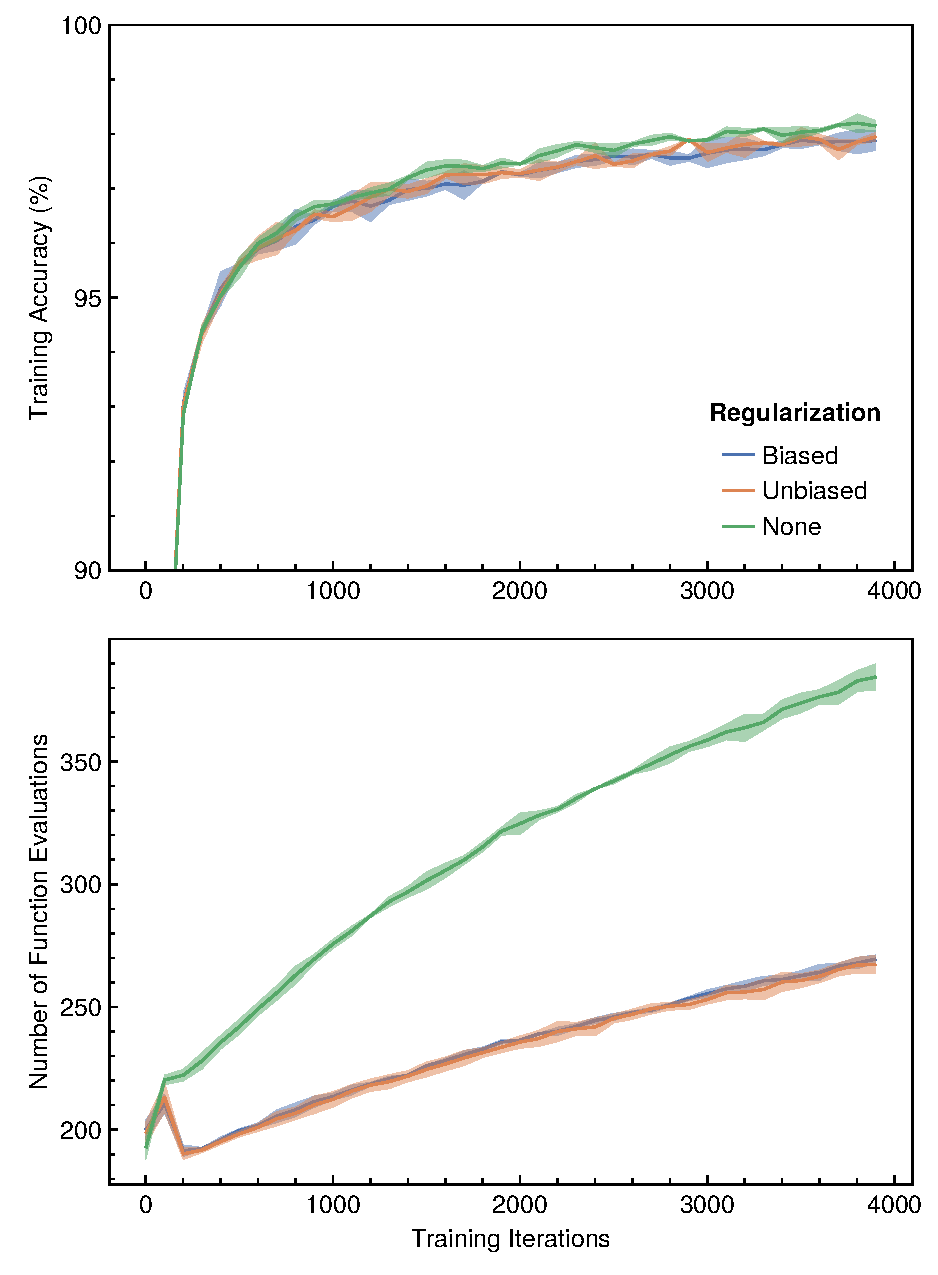
\includegraphics[width=\linewidth]{../figures/local_regularizing_neural_des/mnist_sde.pdf}
    \caption{\textbf{MNIST Classification using Neural SDE}}
    \label{fig:mnist_nsde_localreg}
  \end{minipage}
\end{figure}


\subsection{MNIST Image Classification}
\label{subsec:mnist}

We train a neural differential equation classifier to map flattened MNIST~\citep{lecun1998gradient} images to their corresponding labels.

\begin{table}[t]
  \centering
  \adjustbox{max width=\textwidth}{
    \centering
    \begin{tabular}{llllll}
      \toprule
      \thead{Method}        & \thead{Train Accuracy (\%)} & \thead{Test Accuracy (\%)}      & \thead{Training Time                                                                        \\ (hr)} & \thead{Prediction Time                                           \\ (s / batch)} & \thead{Testing NFE}\\
      \midrule
      Vanilla NODE          & \sdval{99.898}{0.066}       & \sdval{97.612}{0.163}           & \sdval{0.54}{0.001}      & \sdval{0.088}{0.020}     & \sdval{303.559}{3.194}                \\
      STEER\cpaper          & \sdval{100.00}{0.000}       & \sdval{97.94\hp{0}}{0.03\hp{0}} & \sdval{1.31}{0.07\hp{0}} & \sdval{0.092}{0.002}     & \sdval{265.0\hp{0}\hp{0}}{3.46\hp{0}} \\
      TayNODE\cpaper        & \sdval{\hp{0}98.98}{0.06}   & \sdval{97.89\hp{0}}{0.00}       & \sdval{1.19}{0.07}       & \sdval{0.079}{0.007}     & \sdval{\hp{0}80.3\hp{0}\hp{0}}{0.43}  \\
      ERNODE\cpaper         & \sdval{\hp{0}99.71}{0.28}   & \sdval{97.32\hp{0}}{0.06}       & \sdval{0.82}{0.02}       & \sdval{0.060}{0.001}     & \sdval{177.0\hp{00}}{0.00}            \\
      SRNODE\cpaper         & \sdval{100.00}{0.000}       & \sdval{98.08\hp{0}}{0.15}       & \sdval{1.24}{0.06}       & \sdval{0.094}{0.003}     & \sdval{259.0\hp{00}}{3.46}            \\
      Local Unbiased ERNODE & \sdval{99.447}{0.039}       & \sdval{97.526}{0.131}           & \sdval{0.49}{0.002}      & \sdval{0.046}{0.002}     & \sdval{187.961}{1.812}                \\
      Local Biased ERNODE   & \sdval{99.477}{0.051}       & \sdval{97.488}{0.016}           & \sdval{1.12}{0.065}      & \sdval{0.044}{0.002}     & \sdval{182.849}{1.578}                \\
      \addlinespace
      \addlinespace
      Vanilla NSDE          & \sdval{98.27}{0.11}         & \sdval{96.66}{0.16}             & \sdval{2.70}{0.00}       & \sdval{\hp{0}0.51}{0.07} & \sdval{313.86}{2.94}                  \\
      ERNSDE\cpaper         & \sdval{98.16}{0.11}         & \sdval{96.27}{0.35}             & \sdval{4.19}{0.04}       & \sdval{\hp{0}7.23}{0.14} & \sdval{184.67}{2.31}                  \\
      SRNSDE\cpaper         & \sdval{98.79}{0.12}         & \sdval{96.80}{0.07}             & \sdval{8.54}{0.37}       & \sdval{14.50}{0.40}      & \sdval{382.00}{4.00}                  \\
      Local Unbiased ERNSDE & \sdval{98.05}{0.09}         & \sdval{96.57}{0.13}             & \sdval{2.10}{0.01}       & \sdval{\hp{0}0.39}{0.10} & \sdval{228.93}{1.77}                  \\
      Local Biased ERNSDE   & \sdval{98.02}{0.07}         & \sdval{96.44}{0.16}             & \sdval{1.90}{0.00}       & \sdval{\hp{0}0.36}{0.03} & \sdval{230.10}{0.71}                  \\
      \bottomrule
    \end{tabular}
  }
  \caption{\textbf{MNIST Image Classification using Neural DE}: Using local unbiased regularization on neural ODE speeds up training by $\mathit{1.1\times}$ and predictions by $\mathit{1.9\times}$ while reducing the total NFEs to $\mathit{0.619\times}$. Local Biased Regularization tends to slow down training for smaller models on GPU while it further reduces the NFEs by $\mathit{0.602\times}$. For Neural SDE, we observe a similar reduction of NFEs by \timeschange{0.729}{0.733} and a training time improvement of \timeschange{1.28}{1.42}. The best global regularization method gets lower NFEs but overall takes more wall clock than the best performing local regularization method.}
  \label{tab:mnist_node_localreg}
\end{table}

\subsubsection{Neural Ordinary Differential Equation}
\label{subsubsec:mnist_node}

\textbf{Training Details:} We use the same model architecture as described in \citet{kelly2020learning}. Our model comprises of single hidden layered explicit model $f_\theta$ modeling the ODE dynamics followed by a linear classifier $g_\phi$.
% %
% \begin{align}
%     z_\theta(x, t) &= \texttt{tanh}\left( W_1 \times [x; t] + b_1 \right)\\
%     f_{\theta}(x, t) &= \texttt{tanh}\left( W_2 \times [z_\theta(x, t); t] + b_2 \right)\\
%     g_\phi(x, t) &= \sigma\left(W_3 \times x + b_3\right)
% \end{align}
% %
The hidden layer is 100-dimensional. We train with a batch size of 512 for a total of 7500 steps. We use Adam~\citep{kingma2017adam} with a constant learning rate of $0.001$. For error estimate regularization, we exponentially decrease the regularization coefficient from $2.5$ to $1.0$. We use Tsit5~\citep{tsitouras2011runge} as the ODE integrator with an absolute and relative tolerance of $10^{-8}$.\footnote{We note that this is not a realistic tolerance at which image classification models are trained. We use this tolerance to allow a direct comparison to prior works.}

\textbf{Baselines:} We consider a Vanilla Neural ODE trained with the exact aforementioned specifications. All other baselines are directly taken from \citet{pal2021opening}.

\textbf{Results:} We summarize the results in \Cref{tab:mnist_node_localreg} and \Cref{fig:mnist_node_localreg}. Using local regularization speeds up prediction in all cases while it leads to a minor slowdown during training for biased sampling.


\subsubsection{Neural Stochastic Differential Equation}
\label{subsubsec:mnist_nsde}

\textbf{Training Details:} We downsample the flattened images to a 32-dimensional vector before feeding it into the Neural SDE which uses a diffusion model ($f_\theta$) having a 64-dimensional hidden layer and a linear drift model ($g_\phi$). Finally, a linear classifier ($h_\gamma$) predicts the label.
%
% \begin{align}
%     f_\theta(x, t) &= W_2 \times \texttt{tanh}(W_1 \times x + b_1) + b_2\\
%     g_\phi(x, t) &= W_3 \times x + b_3\\
%     h_\gamma(x, t) &= W_4 \times x + b_4
% \end{align}
%
We train our models on CPU with a batch size of $512$ for a total of $4000$ steps. We optimize the weights using Adam~\citep{kingma2017adam} with a constant learning rate of $0.01$. We use SOSRI2 SDE solver~\citep{rackauckas2017adaptive} with a tolerance of $0.14$. We fix our regularization coefficient to be $10^3$. For this experiment, we rely on discrete sensitivity analysis.

\textbf{Baselines:} ERNSDE and SRNSDE results were taken from \citet{pal2021opening}. These were trained for $40$ epochs, nearly equivalent to training for $4000$ iterations.

\textbf{Results:} We summarize the results in \Cref{tab:mnist_node_localreg} and \Cref{fig:mnist_nsde_localreg}. Local regularization improves training and prediction performance while keeping the test accuracy nearly constant.


\subsection{Physionet Time Series Interpolation}
\label{subsec:physionet}


\begin{table}[t]
  \centering
  \adjustbox{max width=\textwidth}{
    \centering
    \begin{tabular}{lllll}
      \toprule
      \thead{Method}        & \thead{Test Loss ($\times 10^{-3}$)} & \thead{Training Time (hr)} & \thead{Prediction Time                        \\(s / batch)} & \thead{Testing NFE}  \\
      \midrule
      Vanilla NODE          & \sdval{3.41}{0.10}                   & \sdval{2.48}{0.22}         & \sdval{0.16}{0.01}     & \sdval{758.0}{25.87} \\
      STEER\cpaper          & \sdval{3.48}{0.01}                   & \sdval{1.62}{0.26}         & \sdval{0.54}{0.06}     & \sdval{699.0}{141.1} \\
      TayNODE\cpaper        & \sdval{4.21}{0.01}                   & \sdval{12.3}{0.32}         & \sdval{0.22}{0.02}     & \sdval{167.3}{11.93} \\
      ERNODE\cpaper         & \sdval{3.57}{0.00}                   & \sdval{0.94}{0.13}         & \sdval{0.21}{0.02}     & \sdval{287.0}{17.32} \\
      SRNODE\cpaper         & \sdval{3.58}{0.05}                   & \sdval{0.87}{0.09}         & \sdval{0.20}{0.01}     & \sdval{273.0}{0.000} \\
      Local Unbiased ERNODE & \sdval{3.64}{0.07}                   & \sdval{2.31}{0.02}         & \sdval{0.09}{0.00}     & \sdval{422.0}{4.580} \\
      Local Biased ERNODE   & \sdval{3.63}{0.08}                   & \sdval{2.12}{0.24}         & \sdval{0.10}{0.01}     & \sdval{463.0}{63.02} \\
      \bottomrule
    \end{tabular}
  }
  \caption{\textbf{Physionet Time Series Interpolation}: Local Regularization reduces NFEs by \timeschange{0.556}{0.610} reducing the prediction timings by \timeschange{1.6}{1.78}. Our methods additionally improve training timings by \timeschange{1.073}{1.167}. We note that the difference in training time compared to (E/S)RNODE methods is due to change in the sensitivity algorithm.}
  \label{tab:physionet_node_localreg}
\end{table}

\textbf{Training Details:} We use the experimental setup for Physionet 2012 Challenge Dataset~\citep{citi2012physionet} from \citet{kelly2020learning}. We use a Latent Neural ODE~\citep{rubanova2019latent} to perform time series interpolation on the dataset. We use the preprocessed dataset from \citet{kelly2020learning} to ensure a fair comparison and independent runs are performed using an 80:20 split of the dataset.

\begin{wrapfigure}{r}{0.5\textwidth}
  \centering
  \vspace{-2em}
  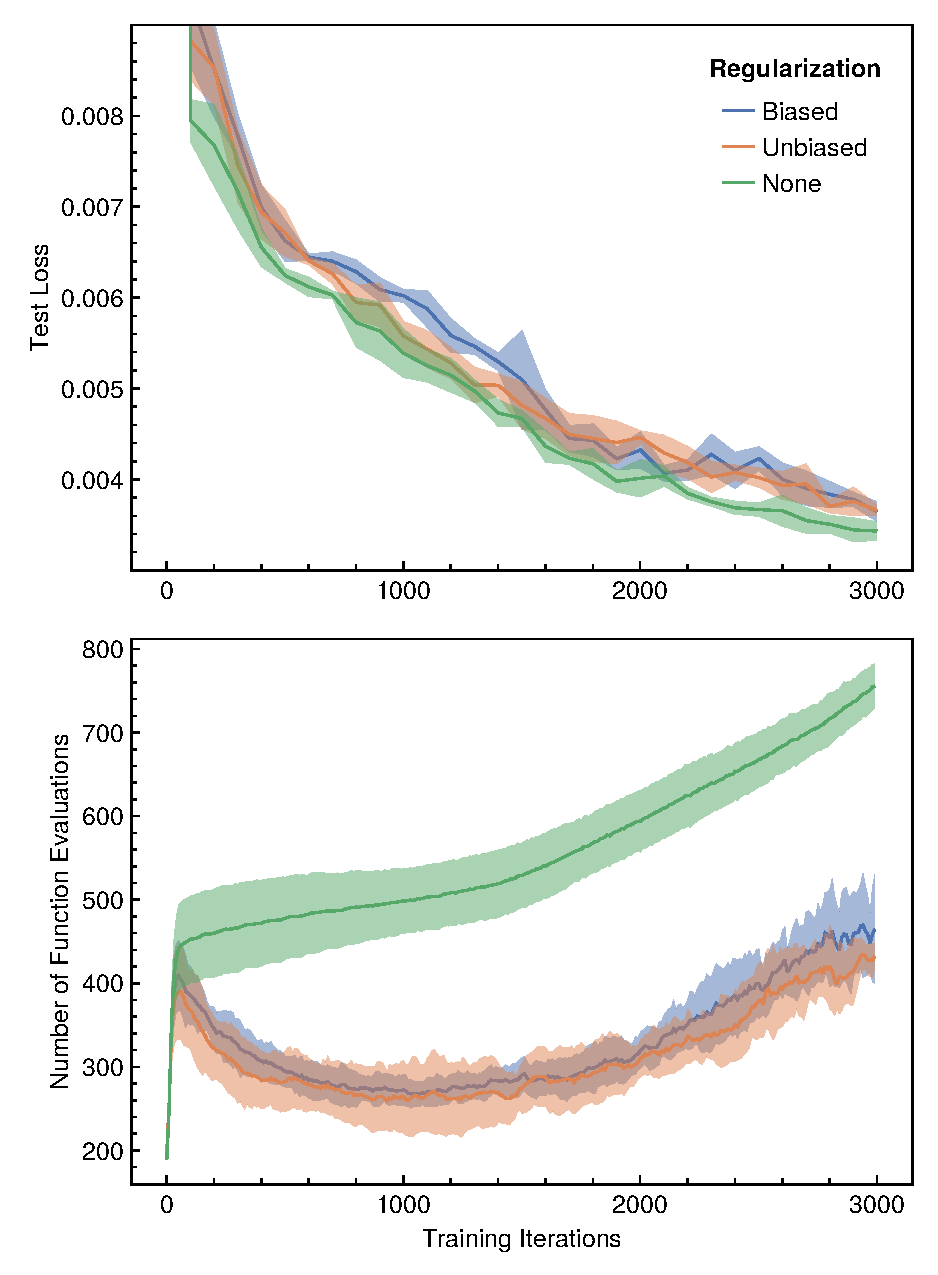
\includegraphics[width=\linewidth]{../figures/local_regularizing_neural_des/physionet.pdf}
  \captionof{figure}{\textbf{Physionet Time Series Interpolation using Latent ODE}}
  \label{fig:physionet_localreg}
  \vspace{-2em}
\end{wrapfigure}

For specific model architecture details, we refer the readers to \citet{pal2021opening}. We train the model for a total of $3000$ iterations using Adamax~\citep{kingma2017adam} with a learning rate of $0.01$ with $10^{-5}$ inverse decay per step. We use a batch size of $512$. We diverge from \citet{pal2021opening}, in using the regularization term as $\left(\eest\right)_{\treg} \cdot |dt|_{\treg}$ instead of the squared regularization term $\sum_j \left(\eest\right)_j^2$. Additionally, we decay the regularization coefficient exponentially from $100$ to $10$ over the $3000$ training iterations.

\textbf{Baselines:} Vanilla NODE was trained with the exact aforementioned configuration. All the other baselines were trained using discrete sensitivity analysis, and the exact details are present in \citet{pal2021opening}.

\textbf{Results:} We summarize the results in \Cref{fig:physionet_localreg} and \Cref{tab:physionet_node_localreg}.

\subsection{CIFAR10 Image Classification}
\label{subsec:cifar10_localreg}


\begin{table}[t]
  \centering
  \adjustbox{max width=\textwidth}{
    \centering
    \begin{tabular}{lllllll}
      \toprule
      \thead{Configuration} & \thead{Method}    & \thead{Train                                                                                                                          \\ Accuracy (\%)} & \thead{Test\\ Accuracy (\%)} & \thead{Training Time\\ (s / batch)} & \thead{Prediction Time\\ (s / batch)} & \thead{Testing\\ NFE}\\
      \midrule
      Standard              & Vanilla           & \sdval{83.683}{1.450}       & \sdval{67.394}{0.849} & \sdval{0.457}{0.018} & \sdval{0.130}{0.013} & \sdval{115.315}{12.136}           \\
                            & Local Unbiased ER & \sdval{83.665}{0.805}       & \sdval{67.678}{0.874} & \sdval{0.399}{0.014} & \sdval{0.096}{0.007} & \sdval{\hp{0}89.048}{\hp{0}7.335} \\
                            & Local Biased ER   & \sdval{83.958}{1.032}       & \sdval{67.745}{0.824} & \sdval{0.555}{0.008} & \sdval{0.088}{0.003} & \sdval{\hp{0}81.301}{\hp{0}1.255} \\
      \addlinespace
      \addlinespace
      Multi-Scale           & Vanilla           & \sdval{92.807}{12.458}      & \sdval{80.048}{6.740} & \sdval{0.572}{0.012} & \sdval{0.170}{0.005} & \sdval{\hp{0}27.616}{\hp{0}0.905} \\
                            & Local Unbiased ER & \sdval{94.159}{\hp{0}9.694} & \sdval{80.432}{5.548} & \sdval{0.641}{0.025} & \sdval{0.175}{0.019} & \sdval{\hp{0}27.760}{\hp{0}0.177} \\
                            & Local Biased ER   & \sdval{99.987}{\hp{0}0.023} & \sdval{83.460}{0.727} & \sdval{0.774}{0.293} & \sdval{0.163}{0.015} & \sdval{\hp{0}26.334}{\hp{0}0.992} \\
      \bottomrule
    \end{tabular}
  }
  \caption{\textbf{CIFAR10 Image Classification using Neural DE}: For the standard Neural ODE, local regularization reduces the NFE by \timeschange{0.705}{0.772}, thereby improving prediction timings by \timeschange{1.35}{1.477}. However, unregularized model training takes $\mathit{0.823\times}$ the time for the biased model. For multi-scale models, the NFE and prediction time improvements are marginal and come at the cost of higher training time.}
  \label{tab:cifar10_node_localreg}
\end{table}

\begin{figure}[t]
  \centering
  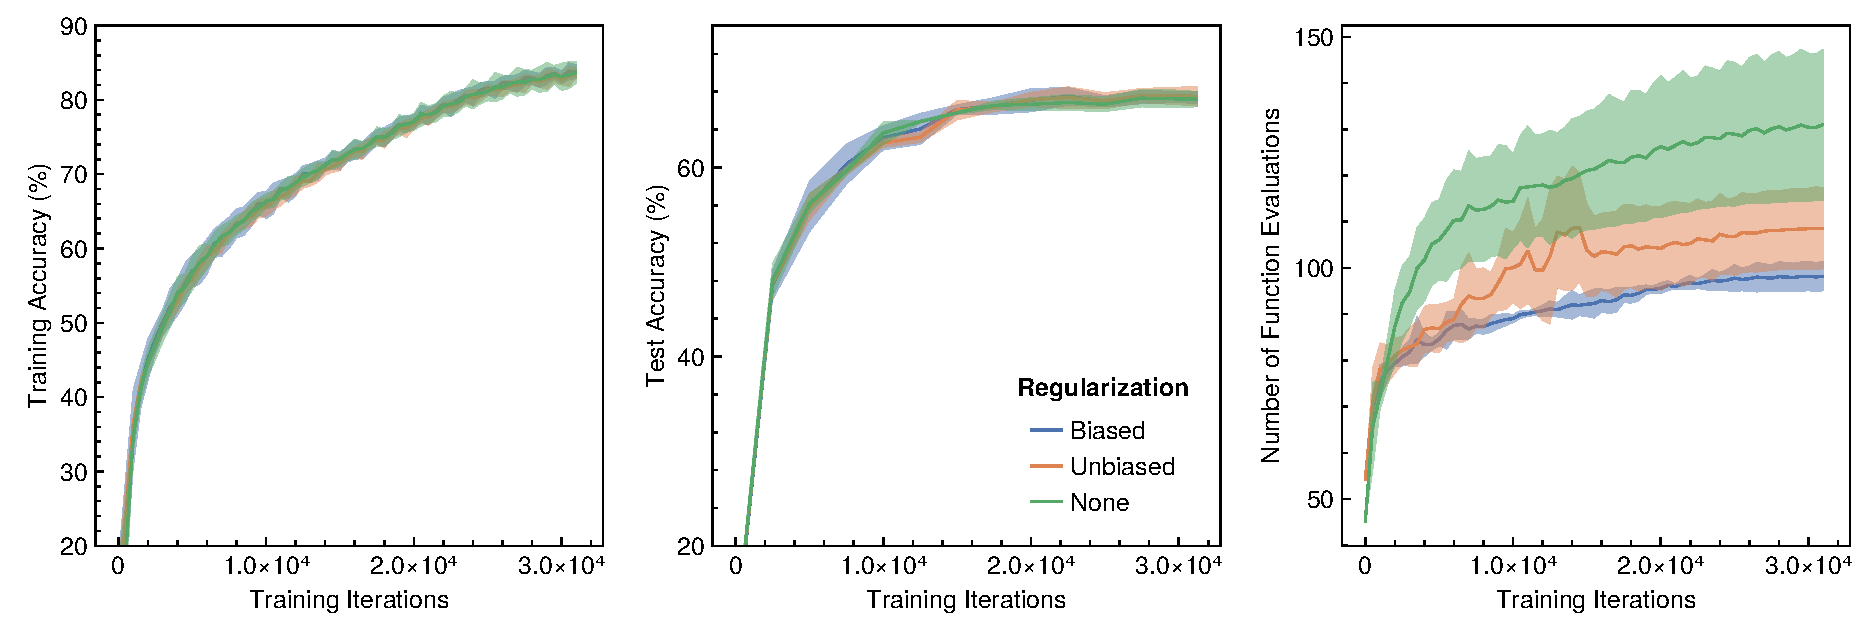
\includegraphics[width=\linewidth]{../figures/local_regularizing_neural_des/cifar10_tiny.pdf}
  \caption{\textbf{CIFAR10 Image Classification using Standard Neural ODE}}
  \label{fig:cifar10_tiny_localreg}
\end{figure}

\subsubsection{Neural Ordinary Differential Equation}
\label{subsubsec:cifar10_node_localreg}

% \input{figures/cifar10_tiny.tex}

\textbf{Training Details:} We use the CNN architecture for CIFAR10 as described in \citet{poli2020hypersolvers}. We train the models for $31250$ steps with Adam~\citep{kingma2017adam} using a cosine-annealing learning rate scheduler from $0.003$ to $0.0001$. We train the models with a batch size of $32$ and keep the regularization coefficient fixed at $2.5$. We use Tsit5~\citep{tsitouras2011runge} with a tolerance of $10^{-4}$.

\textbf{Results:} We summarize the results in \Cref{fig:cifar10_tiny_localreg} and \Cref{tab:cifar10_node_localreg}.

\subsubsection{Multiscale Neural ODE}
\label{subsubsec:cifar10_msnode}

\begin{figure}[t]
  \centering
  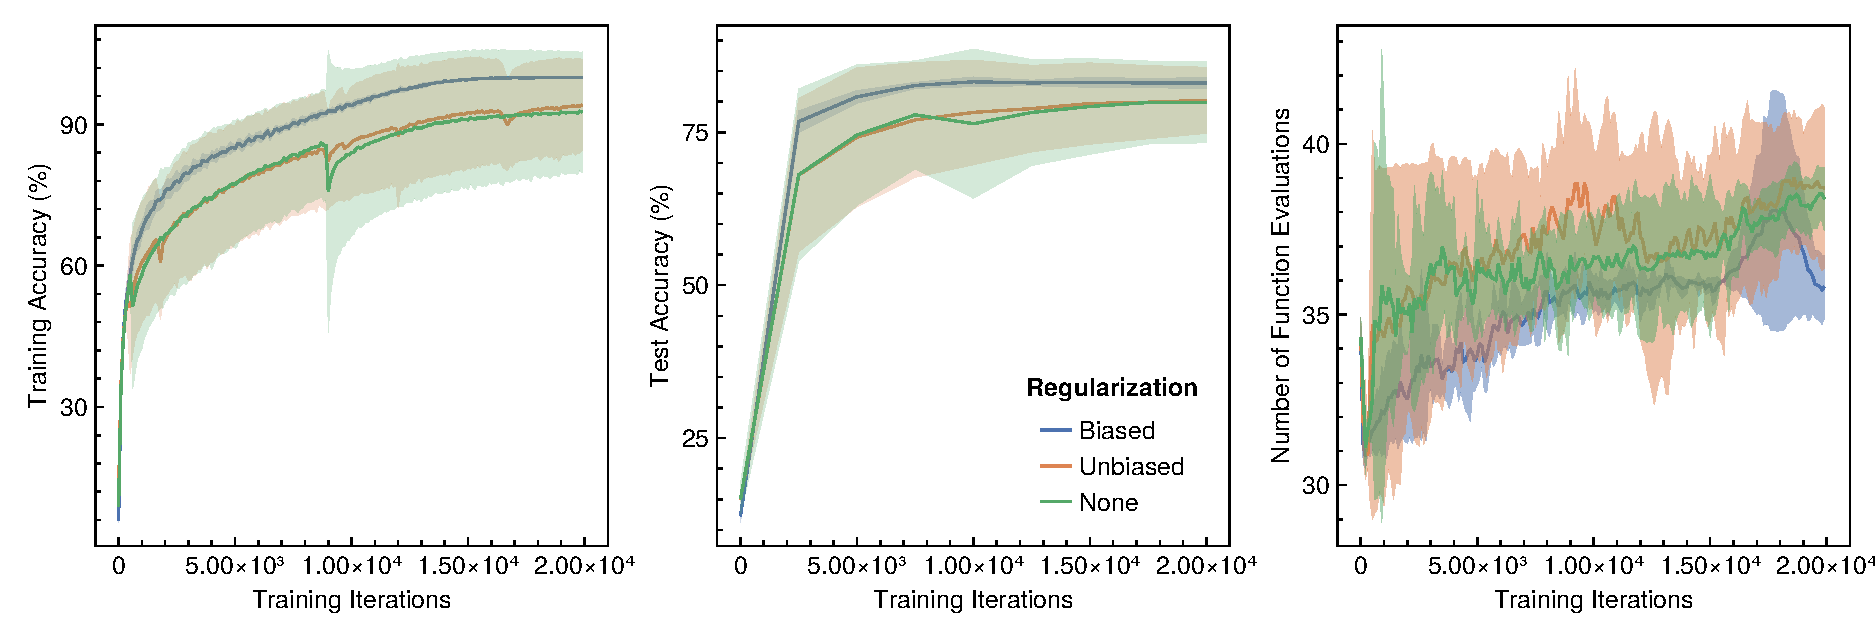
\includegraphics[width=\linewidth]{../figures/local_regularizing_neural_des/cifar10_tiny_msnode.pdf}
  \caption{\textbf{CIFAR10 Image Classification using Multi-Scale Neural ODE}}
  \label{fig:cifar10_tiny_msnode_localreg}
\end{figure}

\textbf{Training Details:} We modify the Tiny Multiscale DEQ architecture for CIFAR10 from \citet{bai_multiscale_2020} as Multiscale Neural ODE with Input Injection. To stabilize the training for larger models, we exponentially increase the regularization coefficient from $0.1$ to $5.0$. We train with a batch size of $128$ using VCAB3~\citep{wanner1996solving} with a tolerance of $0.05$.

\textbf{Results:} We summarize the results in \Cref{fig:cifar10_tiny_msnode_localreg} and \Cref{tab:cifar10_node_localreg}. The benefits from regularization for NFEs and prediction timings seem marginal. However, regularization using biased sampling makes the training dynamics stable as observed in \Cref{fig:cifar10_tiny_msnode_localreg}.


\section{Discussion}
\label{sec:discussion_on_local_regularization_of_neural_des}

In this chapter, we have shown that we can obtain similar properties to global regularization by regularizing dynamical systems at randomly sampled time points. Additionally, this comes with the benefit of not being forced into a specific sensitivity analysis method. We have taken every experiment in \citet{pal2021opening} and empirically showed that our local regularization works at par with global regularization. However, our experiments using stiffness estimate for local regularization did not yield positive results and were not presented in this chapter. Thus, we have demonstrated that we can ``close the blackbox'' and still leverage all the benefits of internal solver heuristics to improve training and predictions of neural differential equations.

\subsection{Limitations}
\label{sec:limitations}

We note the following limitations of our work:
%
\begin{itemize}
  \item Similar to \citet{pal2021opening}, if the objective is to learn the actual dynamical system, our method will not yield proper results. Our method is applicable only when the final state is relevant, i.e., in most classical deep learning tasks.

  \item Regularization introduces a new regularization coefficient hyperparameter which, if not tuned correctly, can lead to unstable dynamics or might negate the scheme's usefulness.
\end{itemize}
%


% Auxiliary Contributions
\part{OPEN SOURCE SOFTWARES}
\label{part:open_source_software}

\chapter{Lux.jl: Bridging Scientific Computing and Deep Learning}
\label{chapter:lux_bridging_scientific_computing_and_deep_learning}

\section{Introduction}
\label{sec:introduction_lux}

Julia already has quite a few well established Neural Network Frameworks – Flux~\citep{innes2018fashionable} \& KNet~\citep{yuret2016knet}. However, certain design elements – \textit{Coupled Model and Parameters} \& \textit{Internal Mutations} – associated with these frameworks make them less compiler and user friendly. Making changes to address these problems in the respective frameworks would be too disruptive for users. In this chapter, we introduce Lux: a neural network framework built completely using pure functions to make it both compiler and autodiff friendly.

The main design principles of Lux include:
%
\begin{enumerate}
  \item \textit{Truly Immutable Models} storing information to construct a layer rather than the parameters and states.
  \item All models are \textit{pure functions} and outputs are completely \textit{deterministic} given the inputs.
  \item Models are decoupled from the parameters and states. This allows us to \textit{perform easy parameter manipulation} like in \textit{Weight Normalization}, \textit{Hypernetworks} and \textit{Spectral Normalization}.
\end{enumerate}
%

\section{Composability via Generic Parameterization}
\label{sec:composability}

One of the distinguishing features of Lux.jl is its generic parameters interface. Lux can accept any special parameter type as long as the parameters are accessible via \textit{getproperty}. This allows Lux to seamlessly interface with packages that are completely agnostic to the specifics of Lux. This is in contrast to most prior works that require glue code for interfacing -- like Flux.jl~\citep{innes:2018} -- or requires reimplementing algorithms in specific Domain Specific Languages (DSLs) -- like Pytorch~\citep{paszke2019pytorch,paszke2017automatic}, JAX~\citep{jax2018github}, Tensorflow~\citep{tensorflow2015-whitepaper}.

Scientific Computing software differ from most modern ML software in that they are designed to operate on arrays, while ML software operate on deeply nested structures. This is a fundamental difference that makes it difficult to interface between the two. However, Lux.jl is designed to be agnostic to the underlying data structure. In this section, we will demonstrate several examples interfacing Lux with Scientific Computing frameworks solving Neural ODEs, Physics Informed Neural Networks and Optimization Problems.

\subsection{Neural Differential Equations}
\label{subsec:differential_equations_lux}

In this thesis, we have described Neural ODEs in great depth. However, for physics based modelling we often need to rely on higher order differential equations. In this section, we will describe how to model a second order differential equation using Lux.jl and OrdinaryDiffEq.jl. We will attempt to model the acceleration of a system using a Neural Network\footnote{We have modified this example from \url{https://docs.sciml.ai/SciMLSensitivity/stable/examples/ode/second_order_neural/}}:
%
\begin{equation}
  \frac{d^2u}{dt^2} = \texttt{NN}(u)
\end{equation}
%

\inputminted[linenos, breaklines, fontsize=\scriptsize, frame=single, framesep=10pt]{julia}{../code/diffeq.jl}

\begin{figure}
  \centering
  \begin{subfigure}[c]{0.48\linewidth}
    \centering
    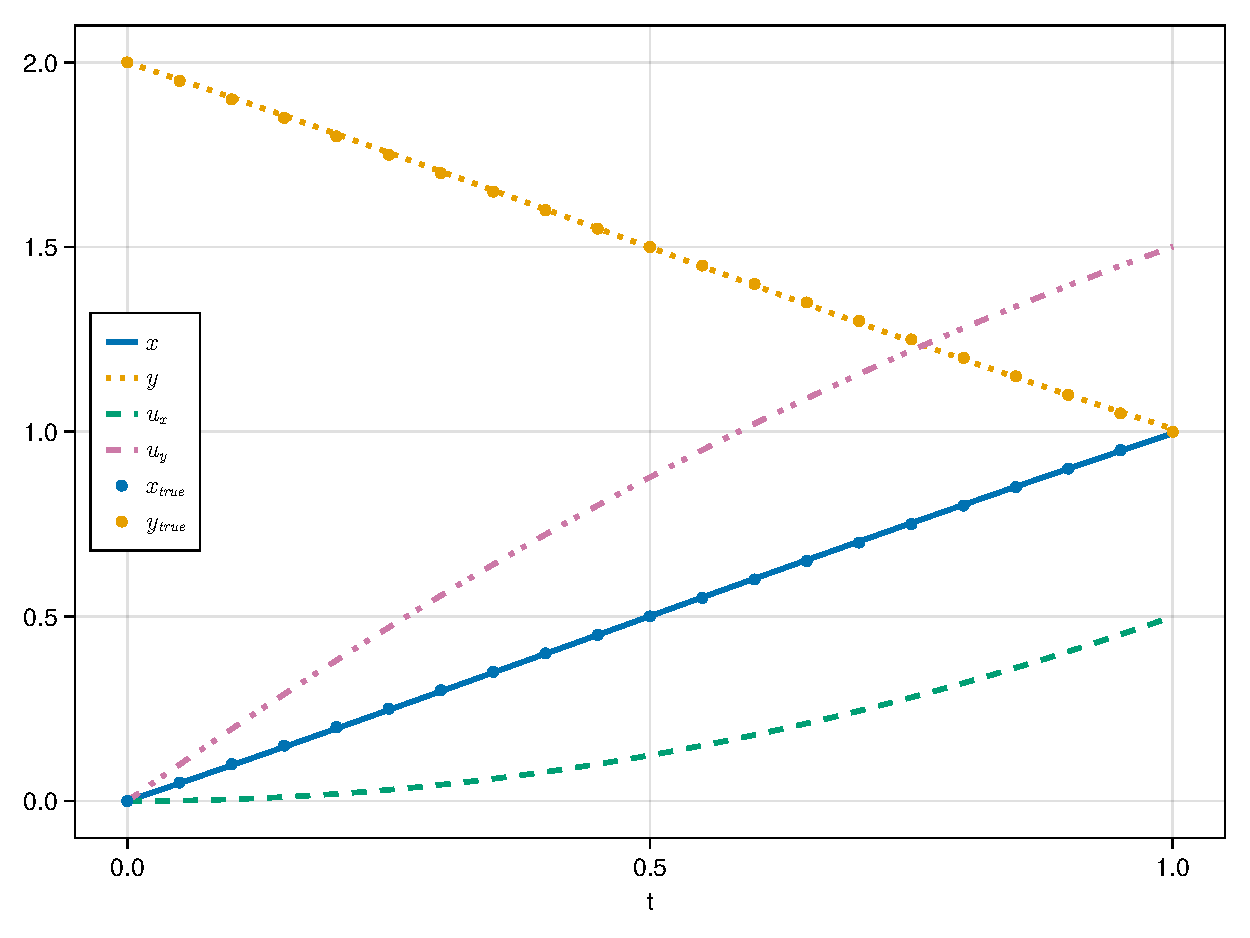
\includegraphics[width=\textwidth]{../figures/lux/diffeq_plot.pdf}
    \caption{\textbf{Learning $2^{nd}$ order differential equation with Lux.jl.}}
    \label{fig:lux_diffeq_plot}
  \end{subfigure}
  \hfill
  \begin{subfigure}[c]{0.48\linewidth}
    \centering
    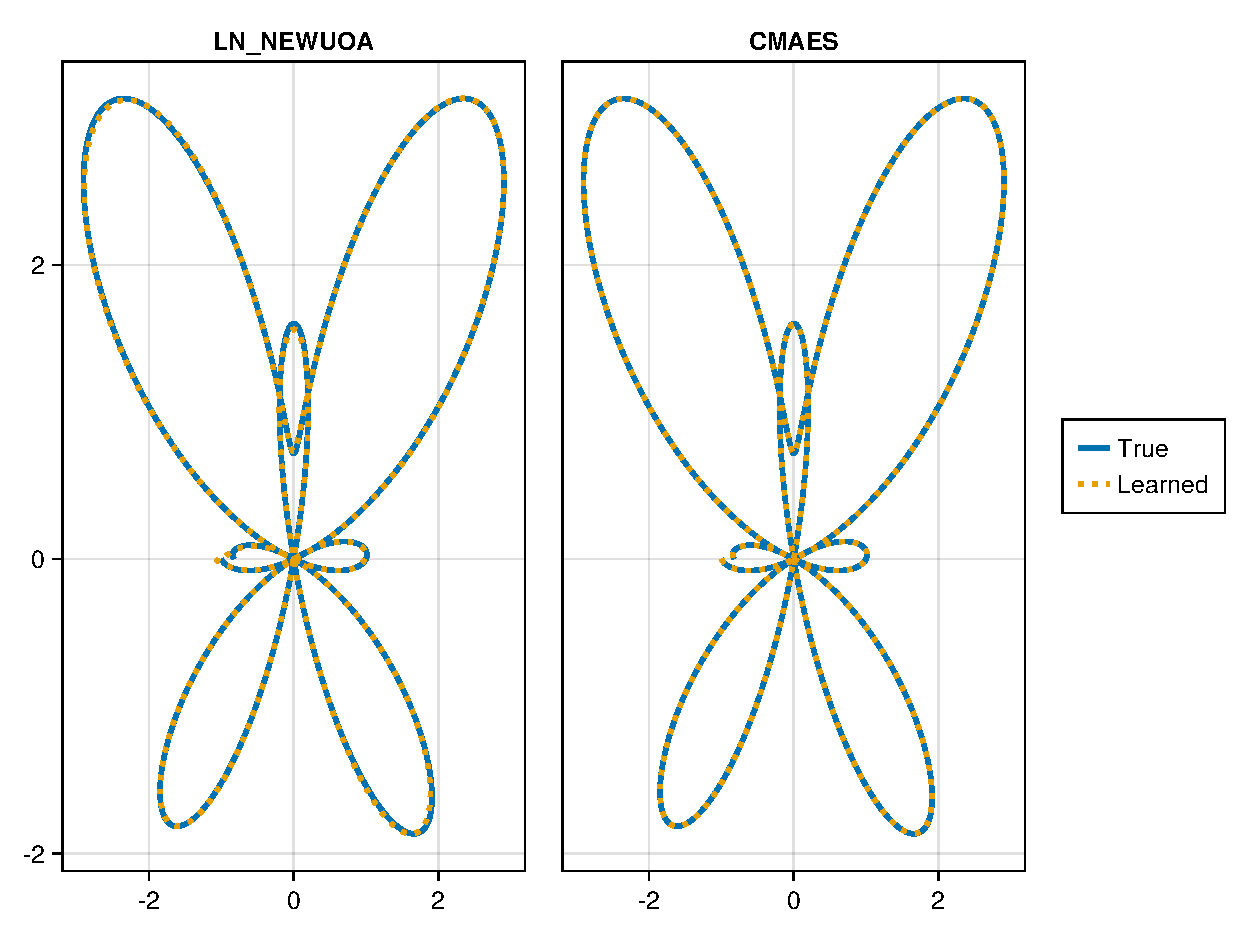
\includegraphics[width=\textwidth]{../figures/lux/gfopt_plot.pdf}
    \caption{\textbf{Gradient Free Optimization to train a neural network} to approximate the function $r(\theta) = e^{sin(\theta)} - 2cos(4\theta) + sin\left(\frac{2\theta - \pi}{12}\right)^5$.}
    \label{fig:lux_gfopt_plot}
  \end{subfigure}
\end{figure}

% \begin{figure}[t]
%   \centering
%   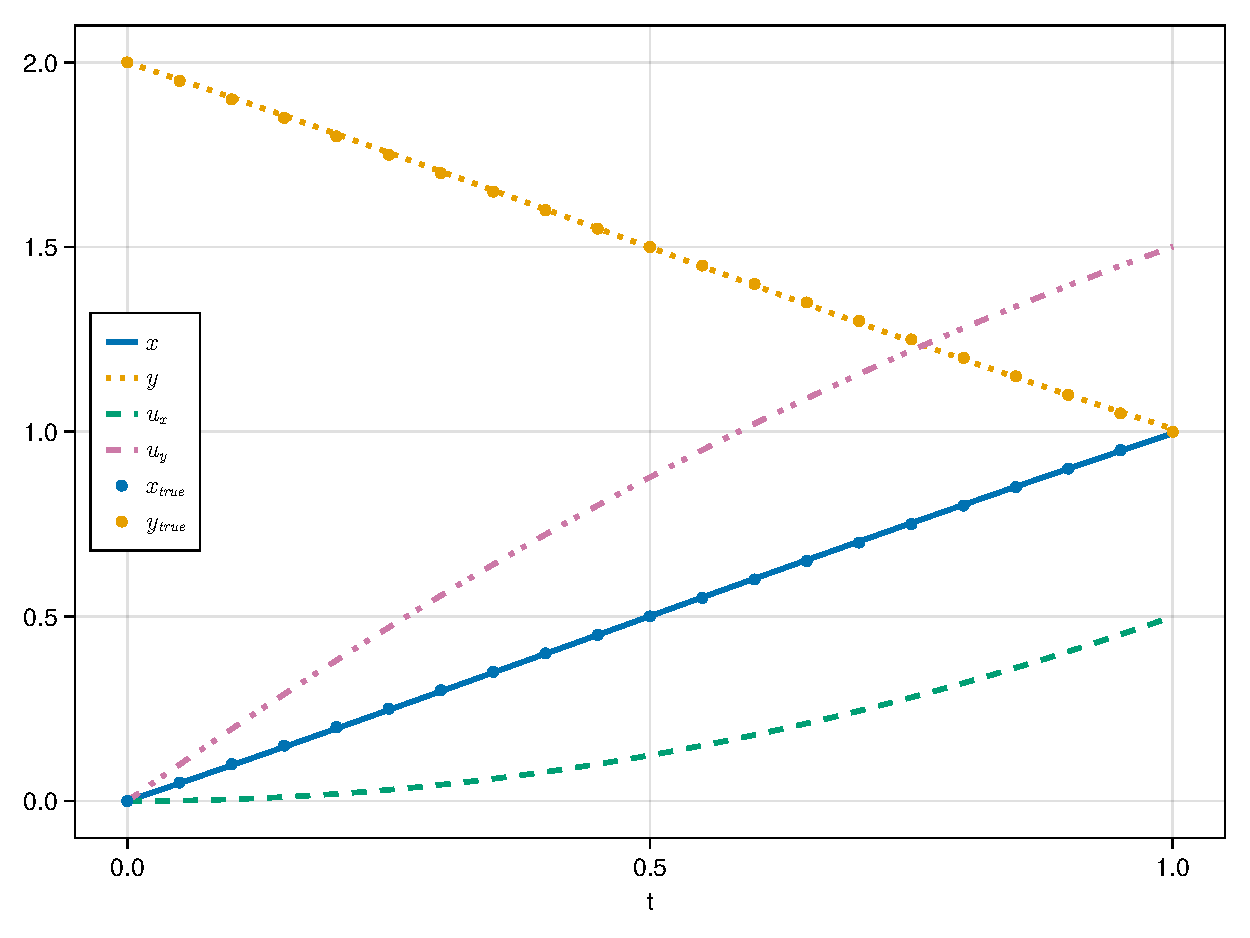
\includegraphics[width=0.5\textwidth]{../figures/lux/diffeq_plot.pdf}
%   \caption{\textbf{Learning $2^{nd}$ order differential equation with Lux.jl.}}
%   \label{fig:lux_diffeq_plot}
% \end{figure}

\Cref{fig:lux_diffeq_plot} shows that our model is able to accurately learn the dynamics of the system from a few discrete data points. This is a very simple example, but it demonstrates the composability of Lux.jl and DifferentialEquations ecosystem.

\subsection{Gradient Free Optimization Algorithms}
\label{subsec:evolutionary_alg_lux}

Lux allows the parameters of a complicated neural network to be represented as a flattened vector. This allows it to interface directly with optimization packages without any glue code. In this example, we will train a neural network with gradient-free optimization algorithms to learn the function:
%
\begin{align}
  r(\theta)              & = e^{sin(\theta)} - 2cos(4\theta) + sin\left(\frac{2\theta - \pi}{12}\right)^5 \\
  \texttt{where } \theta & \in [0, 2\pi]
\end{align}
%
We will use algorithms implemented in packages that are agnostic to the specifics of Lux\footnote{Note that these are not the most efficient algorithms to solve the problem, but these simply demonstrate the composability of Lux.}:
%
\begin{itemize}
  \item Covariance Matrix Adaptation Evolutionary Strategy (CMAES)~\citep{hansen2016cma} from CMAEvolutionStrategy.jl.
  \item LN\_NEWUOA~\citep{powell2006newuoa} from NLopt.jl~\citep{johnson2021nlopt}. Since Lux allows flattened parameters we can easily interoperate with NLopt which is a C library.
\end{itemize}
%

\inputminted[linenos, breaklines, fontsize=\scriptsize, frame=single, framesep=10pt]{julia}{../code/gfopt.jl}

% \begin{figure}[t]
%   \centering
%   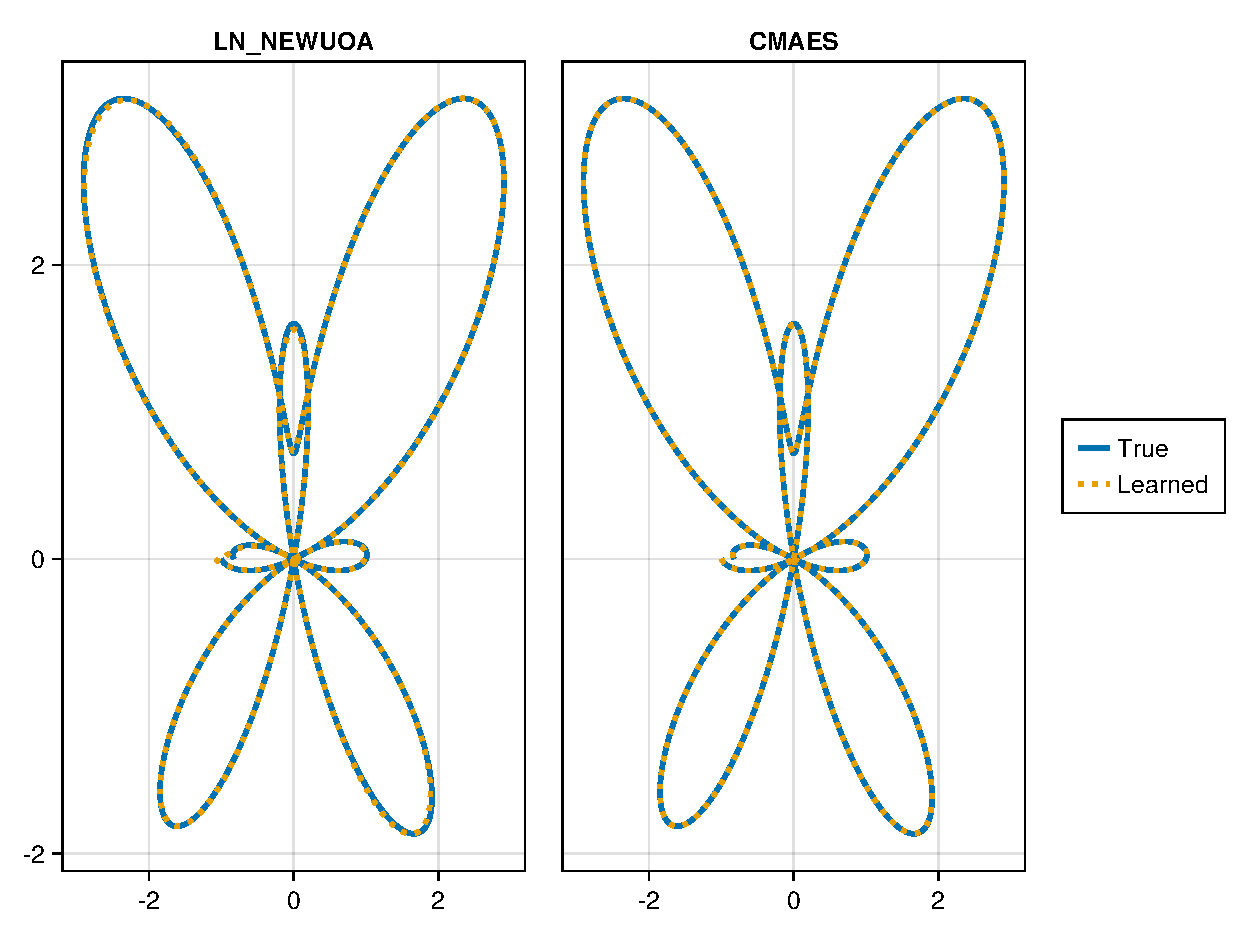
\includegraphics[width=0.8\textwidth]{../figures/lux/gfopt_plot.pdf}
%   \caption{\textbf{Gradient Free Optimization to train a neural network} to approximate the function $r(\theta) = e^{sin(\theta)} - 2cos(4\theta) + sin\left(\frac{2\theta - \pi}{12}\right)^5$.}
%   \label{fig:lux_gfopt_plot}
% \end{figure}

\subsection{Physics Informed Neural Networks}
\label{subsec:physics_informed_neural_networks_lux}

Lux.jl supports PINNs using NeuralPDE.jl~\citep{zubov2021neuralpde}. In this example, we will solve the Kuramoto–Sivashinsky equation\footnote{This example has been adapted from \url{https://docs.sciml.ai/NeuralPDE/stable/examples/ks/}}:
%
\begin{align}
  \frac{\partial \func{u}{x, t}}{\partial t} + \func{u}{x, t} \cdot \frac{\partial \func{u}{x, t}}{\partial x} + \alpha \cdot \frac{\partial^2 \func{u}{x, t}}{\partial x^2} + \beta \cdot \frac{\partial^3 \func{u}{x, t}}{\partial x^3}  + \gamma \cdot \frac{\partial^4 \func{u}{x, t}}{\partial x^4} = 0
\end{align}
%
For $\alpha = \gamma = 1$ and $\beta = 4$, we have the exact analytic solution:
%
\begin{align}
   & \func{u_e}{x, t} = 11 + 15 \tanh \theta - 15 \tanh^2 \theta - 15 \tanh^3 \theta \\
   & \texttt{where } \theta = t - \frac{x}{2}
\end{align}
%
The initial and boundary conditions are given by:
%
\begin{align}
   & \func{u}{x, 0} = \func{u_e}{x, 0}                                                             \\
   & \func{u}{-10, t} = \func{u_e}{-10, t}                                                         \\
   & \func{u}{10, t} = \func{u_e}{10, t}                                                           \\
   & \func{\frac{\partial u}{\partial x}}{-10, t} = \func{\frac{\partial u_e}{\partial t}}{-10, t} \\
   & \func{\frac{\partial u}{\partial x}}{10, t} = \func{\frac{\partial u_e}{\partial t}}{10, t}
\end{align}
%

\begin{figure}[t]
  \centering
  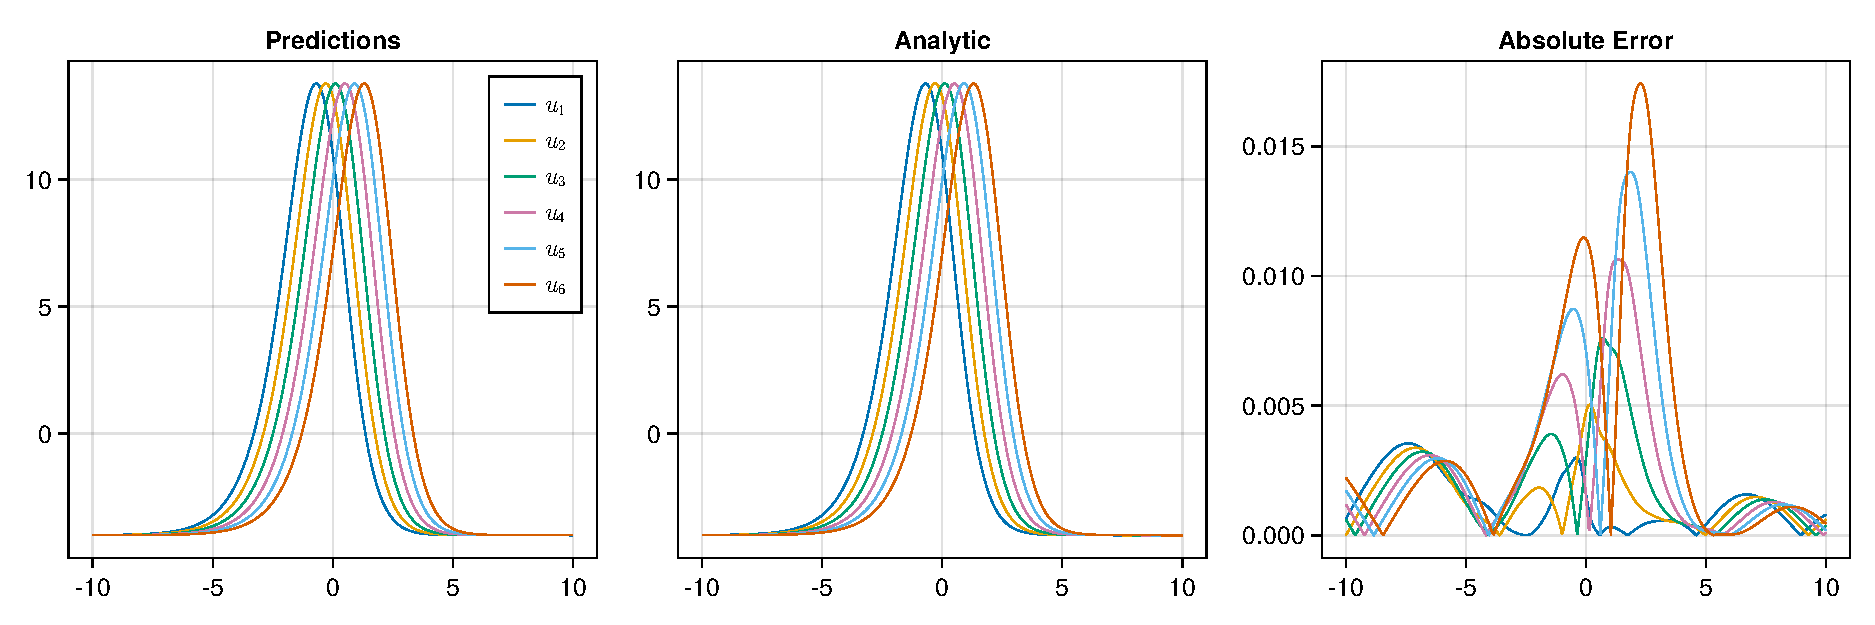
\includegraphics[width=\textwidth]{../figures/lux/pinn_plot.pdf}
  \caption{\textbf{Physics Informed Neural Networks using Lux} for solving Kuramoto–Sivashinsky equation.}
  \label{fig:lux_pinn_plot}
\end{figure}

\inputminted[linenos, breaklines, fontsize=\scriptsize, frame=single, framesep=10pt]{julia}{../code/pinn.jl}

\Cref{fig:lux_pinn_plot} demonstrates that our PINN can solve the Kuramoto–Sivashinsky equation with high accuracy.

\section{Discussion}
\label{sec:discussion_lux}

In this chapter, we have introduced a new neural network framework in Julia. We designed the framework to be modular and composable. We demonstrated the composability of Lux.jl by showing how it can be used with other packages in the Julia ecosystem. We also showed that Lux.jl can be used to solve a variety of problems. Despite being in early days of development, Lux.jl is already being used extensively in research projects and being extended by the open-source community.

\subsection{Current Limitations}
\label{subsec:current_limitations}

Lux.jl has the following known limitations, most of which are being actively worked upon:
%
\begin{itemize}
  \item Lux.jl is not the fastest framework for training small neural networks on CPU. For smaller architectures, \href{https://github.com/PumasAI/SimpleChains.jl}{SmallChains.jl} is the fastest option.
  \item Lux.jl shares the same backend as Flux.jl and hence migration from Flux to Lux doesn't speed up user code. However, a new backend \href{https://github.com/LuxDL/LuxLib.jl}{LuxLib.jl} is under development which should be faster than Flux.jl's backend.
  \item Lux.jl is currently tested to work on CPU and NVIDIA CUDA GPUs. Support for AMD GPUs is being worked upon.
  \item Nested Reverse Mode differentiation of Lux models is not supported yet.
\end{itemize}
%

\chapter{DeepEquilibriumNetworks.jl: Implicit Machine Learning with O(1) Backpropagation}
\label{chapter:deep_equilibrium_networks_software}

% Conclusion & Future Work
\part{CONCLUSIONS AND FUTURE WORK}
\label{part:conclusion_and_future_work}

\chapter{Conclusion}
\label{chapter:conclusion}

In this thesis, we have two objectives. Firstly, we have attempted to provide an overview of numerical methods literature for deep learning practitioners and researchers. By reviewing traditional numerical methods, we attempt to show how we can leverage domain specific knowledge of solver internals to accelerate training of Neural Differential Equations. Additionally, we discuss non-linear solvers to expose readers to the internals of deep equilibrium models and draw parallels between Neural ODEs and deep equilibrium models.

Additionally in this thesis we have introduced two novel training strategies for accelerating Neural Differential Equations:
%
\begin{enumerate}
    \item Building upon the prior works on discrete deep equilibrium networks~\citep{bai_deep_2019,bai_multiscale_2020}, we propose continuous deep equilibrium methods~\citep{pal2022mixing} which are a special case for Neural ODEs with the integration end-point being $\infty$. Interestingly, we demonstrate that integrating Neural ODEs to $\infty$ paradoxically, simplifies the back-propagation thereby accelerating training significantly.
    
        Additioanlly, we propose methods like Skip DEQ and Skip Regularized DEQs which further accelerate training by attempting to predict the steady-state or simplify the learned dynamics.

    \item Next, we provide a detailed review on \citet{pal2021opening}, and discuss the major shortcomings of discrete sensitivity analysis methods. We then propose a novel local regularization method for Neural ODEs which is inspired by the global regularization method proposed in \citet{pal2021opening}. We demonstrate that our proposed method is able to achieve similar performance as global regularization methods while being significantly easier to integrate into existing code-bases.
\end{enumerate}
%

\section*{Future Works}
\label{sec:future_works}

In this thesis, we have described how to accelerate the training and prediction timings of Neural Differential Equations. However, despite these advances we note that these models are still not competitive to standard explicit models for classical deep learning tasks. But despite their shortcomings in traditional tasks, we note that implicit models still hold immense value in areas where it is hard to retrofit explicit models. For example, in the case of physical simulations, implicit models like Hamiltonian Neural Networks~\citep{greydanus2019hamiltonian}, Lagrangian Neural Networks~\citep{cranmer2020lagrangian}, etc. can directly conserve physical laws. Continuous Normalizing Flows~\citep{chen2018neural} and FFJORD~\citep{grathwohl2018ffjord} are able to perform density estimation via normalizing flows without the need for specific invertible architectures. Latent ODE models~\citep{rubanova2019latent} can successfully learn time-series models from irregularly spaced data. Hence, while implicit models might not be competitive in traditional domains like image classification, we believe that they are already competitive in several niche domains.

Another domain where implicit models can be of immense value are in enforcing hard constraints on the output space of the neural networks. We have already seen convex optimization layers~\citep{agrawal2019differentiable} for enforcing convex constraints in neural network outputs. However, we believe we can use implicit models like Neural Boundary Value Problems (BVPs) for enforcing arbitrary equality constraints on the output space. Essentially, solving general BVPs involve solving a Nonlinear Problem minimizing a residual to match boundary conditions. Therefore, similar to DEQs their back-propagation is given by a simple linear equation that can be efficiently solved using Matrix-Free Krylov methods.

Furthermore, we can enforce properties like complementarity on the output space in the form of Neural Nonlinear Complementarity Models:
%
\begin{align}
    &x^T \func{f}{x} = 0\\
    & x \geq 0 \qquad \func{f}{x} \geq 0
\end{align}
%
Despite these strong inductive biases in these models, we note that the back-propagation through these models is still well defined and extremely simple. Most of these models can be reduced to Nonlinear Problems and hence back-propagation through these models is as simple as solving a Linear Problem. We believe that reformulation of common constraints as Nonlinear Problems opens up a pandora's box of possibilities for implicit models in enforcing hard constraints.

% Appendix (if Any)

\SgIncludeBib{references}

\end{document}